\documentclass[ITR,BA,english,final,]{LSR_thesis} 
\graphicspath{{pics/}}

%% Options:
%% LSR: LSR Template with Prof. Buss as default
%% ITR: ITR Template with Prof. Hirche as default

%% BA: Bachelorarbeit / Bachelor thesis
%% MA: Masterarbeit / Master thesis
%% HS: Hauptseminar / Scientific seminar
%% PP: Projektpraktikum / practical course
%% IP: Ingenieurpraxis
%% FP: Forschungspraxis
%% SeA: Semesterarbeit (MW)

%% english
%% german

%% final
%% intermediate

%% tutorial -> remove flag such that help files and todos are removed

%%% last changes: 7.02.2019 (v.gabler@tum.de)

%------------------------------------------------%
%_________CUSTOMIZE LATEX ONLY IN customize.tex!_% 
%_________ DO NOT MODIFY THE TEMPLATE!___________%
%________________________________________________%
% add customize first so you can access your commands in gloss, or fuse both into one file
%%%%%%%%%%%%%%%%%%%%%%%%%%%%%%%%%%%%%%%%%%%%%%%%%%%%%%%%%%%%%%
% CUSTOMIZING Tex-File for students to be adjusted as needed %
%%%%%%%%%%%%%%%%%%%%%%%%%%%%%%%%%%%%%%%%%%%%%%%%%%%%%%%%%%%%%%
%%%%%%%%%%%%%%%%%%%%%
% CUSTOM PACKAGES	%
%%%%%%%%%%%%%%%%%%%%%
\usepackage{tikz}
\usepackage{pgfplots}
\usepackage{amsmath,amssymb,amsfonts}
\usepackage{mathtools}
\usepackage{commath}
\usepackage{algorithmic}
\usepackage{algorithm}
\usepackage{caption}
%\usepackage{subcaption}
%%%%%%%%%%%%%%%%%%%%%
% CUSTOM COMMANDS	%
%%%%%%%%%%%%%%%%%%%%%
% e.g. Math conventions as vectors, Matrices, sets
\renewcommand{\vec}[1]{\mathbf{\MakeLowercase{#1}}}
\newcommand{\Mat}[1]{\mathbf{\MakeUppercase{#1}}}
%\newcommand{\set}[1]{\boldsymbol{#1}}
\newcommand*{\txtspc}[1]{\phantom{.}#1\phantom{.}}%
% e.g. use differenc layers in tikz
\pgfdeclarelayer{background}
\pgfdeclarelayer{nodelayer}
\pgfdeclarelayer{edgelayer}
\pgfdeclarelayer{foreground}
\pgfsetlayers{background,edgelayer,nodelayer,main,foreground}
%%%%%%%%%%%%%%%%%%%%%
% HYPHENATIONS 		%
%%%%%%%%%%%%%%%%%%%%%
\hyphenation{Lya-pu-nov}

 % add custom commands etc in this file 
% %%%%%%%%%%%%%%%%%%%%%%%%%%%%%%%%%%%%%%%%%%%%%%%%%%%%%%%%%%%%%%
% NOTE: Using this is optional
% 	Nonetheless, feel free to include this file and adjust the 
% 	examples below as needed
%   
% Questions, feedback and improvements:
%	-> https://git.lsr.ei.tum.de/students/student-templates/issues
% ATTENTION:
% 	- Keep in mind that thif file uses the \vec and \mat commands
% 	 	which are defined in customize.tex!
%	- add glsaddall if you want all of the elements in gloss.aux
%		being printed into your list of acronyms.
% Further reading:
%	https://ctan.org/pkg/glossaries?lang=en
%%%%%%%%%%%%%%%%%%%%%%%%%%%%%%%%%%%%%%%%%%%%%%%%%%%%%%%%%%%%%%

% include packages
\usepackage{setspace}
\usepackage{filecontents}
% for sharelatex, the indexing using xindy:
% 	http://xindy.sourceforge.net/doc/faq-1.html#ss1.2
% is not available, thus the adjustments below ar necessary
%% Adjust Flag for Sharelatex
\newif\ifShareLatex 
%\ShareLatextrue            	% if you work in sharelatex: https://sharelatex.tum.de
\ShareLatexfalse          		% if you work locally

\ifShareLatex
    \usepackage[acronym, style=alttree, shortcuts, toc=true, nomain, nonumberlist]{glossaries}
    \renewcommand{\makeglossaries}{\makenoidxglossaries}
    \renewcommand{\printglossary}{\printnoidxglossary}
\else
    \usepackage[acronym,style=alttree, toc=true, shortcuts, xindy, nomain, nonumberlist]{glossaries}
    \RequirePackage[xindy]{imakeidx}
\fi

%%%%%%%%%%%%%%%%%%%%%%%%%%%%%%%%%%
% DEFINE HEADINGS AND CATEGORIES %
%%%%%%%%%%%%%%%%%%%%%%%%%%%%%%%%%%
% preferable use a command, to adjust the Capitalization 
% for the header section of fancyhdr automatically
\newcommand{\Symbols}{List of Symbols}
\newcommand{\Notation}{Notation}
\newglossary{symbols}{sym}{sbl}{\Symbols}
\newglossary{notation}{not}{nt}{\Notation}
% set width of first row
\glssetwidest{THISWIDE}     % adjust length as needed

%%%%%%%%%%%%%%%%%%%%%%%%%%%%%
% DEFINE ACRONYMS/GLOSSARY	%
%%%%%%%%%%%%%%%%%%%%%%%%%%%%%
\makeglossaries % don't remove this
\begin{filecontents}{gloss.aux}
	%===========%
	% ACRONYMS	%
	%===========%
	\newacronym{MPC}{MPC}{model-predictive control}
	\newacronym{BIBO}{BIBO}{bounded-input bounded-output}
	\newacronym{HRC}{HRC}{Human-Robot Collaboration}
	%============%
	% SYMBOLS	%
	%===========%
	\newglossaryentry{control}{type=symbols,
		sort={control},
		name={\ensuremath{\vec{u}}},
		description={control input vector}
	}
	%============%
	% NOTATION	%
	%===========%
	\newglossaryentry{vector}{type=notation,
		sort={vector},
		name={\ensuremath{\vec{x}_n}},
		description={$n$-dimensional vector named $x$}
	}	
	\newglossaryentry{matrix}{type=notation,
		sort={vector-matrix},
		name={\ensuremath{\Mat{x}_{m\times n}}},
		plural={matrices},
		user1={Mat},
		description={\ensuremath{m\times n} dimensional Matrix  named \ensuremath{X}}
	}	
\end{filecontents}
\loadglsentries{gloss.aux}

%%%% Add GLOSSARIES at end of thesis
\newcommand{\AddMyGloss}{
	\ifLSRITRtutorial
		\glsaddall 
	\fi
	\renewcommand{\glsglossarymark}[1]{}
   	\printglossary[type=acronym]
	\markboth{\MakeUppercase{acronyms}}{\MakeUppercase{acronyms}}
  	\ifdefined\Symbols
		\printglossary[type=symbols, nogroupskip]
		\markboth{\MakeUppercase{\Symbols}}{\MakeUppercase{\Symbols}}
	\fi
	\ifdefined\Notation
		\printglossary[type=notation, nogroupskip]
		\markboth{\MakeUppercase{\Notation}}{\MakeUppercase{\Notation}}
	\fi
}

		% add your glossary in this file 


%_______Start_Document______________________________________
\begin{document}
%%%%%%%%%%%%%%%%%%%%%%%%%%%%%%%%%%%%%%%%%%%%%%%%%%%%%%%%%%%%%%%
%%%%%%%%%%%%%%%%%%% title page %%%%%%%%%%%%%%%%%%%%%%%%%%%%%%%%
%%%%%%%%%%%%%%%%%%%%%%%%%%%%%%%%%%%%%%%%%%%%%%%%%%%%%%%%%%%%%%%
%% for an english theis. The title:
\title{Constrained Optimal Coverage Control of a Multi-Unicycle System}
%% Für deutsche Arbeiten: Deutscher Titel:
%\title{Die Antwort auf Alles und Mehr - Ein Trauerspiel in 4 Akten}
% and English translation (optional)
%\titletranslation{Die Verwendung eines Deutschen Untertitels obliegt der Verantwortung der entsprechenden Betreuer}
% data about YOU!:
\student{Khanh Le} 			%% your name
\studtitle{Nhan} 			%% Bachelor of Arts, Dr.~phil, etc.
\street{Adelheidstrasse 13}			%% your address
\city{80798 Munich}								%		"
\phone{+4915252654118}			%% your telephone-no.

%% if more students are involved (e.g. PP) 
%--the following parted is not tested ---
% please report bugs to v.gabler@tum.de 
%\studenttwo{Zweiter Student}
%\studtitletwo{} 
%\studentthree{} 
%\studtitlethree{} 
%\studentfour{} 
%\studtitlefour{} 
%-----------------------------------------
\supervisor{Dr. Qingchen Liu \& M.Sc Zengjie Zhang}			%% your supervisor
\finalrep{20.07.2020}						%% final presentation / date

\maketitle
%%%%%%%%%%%%%%%%%%%%%%%%%%%%%%%%%%%%%%%%%%%%%%%%%%%%%%%%%%%%%%%
%%%%%%%%%%%%%%%%%%%%%%%%%%%%%%%%%%%%%%%%%%%%%%%%%%%%%%%%%%%%%%%

\newpage
\cleardoublepage
\ifLSRITRtutorial
		\phantom{u}
		\phantom{1}\vspace{6cm}
	\begin{center}
		\add[inline]{In your final hardback copy, replace this page with the signed exercise sheet.}
		\vspace{3cm}
		\todo[inline,color=red!70]{Before modifying this document, READ THE INSTRUCTIONS AND GUIDELINES!}
	\end{center}
\else
	% in case you want to add the PDF directly add the task description in the include directory
	\includepdf[pages=1]{./include/Thesis.pdf}
\fi
\newpage


%%%%%%%%%%%%%%%%%%%%% Declaration %%%%%%%%%%%%%%%%%%%%%%%%%%%%%%%%%
\phantom{u}
\phantom{1}\vspace{6cm}
\begin{center}
	DECLARATION \\
\end{center}
I declare that the work in this bachelor's thesis in electrical and computer engineering is my own work and I have documented all sources and material used.

%%%%%%%%%%%%%%%%%%%%%%%%%%%%%%%%%%%%%%%%%%%%%%%%%%%%%%%%%%%%%%%
%%%%%%%%%%%%%%%%%%%%% abstract %%%%%%%%%%%%%%%%%%%%%%%%%%%%%%%%
%%%%%%%%%%%%%%%%%%%%%%%%%%%%%%%%%%%%%%%%%%%%%%%%%%%%%%%%%%%%%%%
\topmargin5mm
\textheight220mm
\pagenumbering{arabic}
\phantom{u}
\begin{abstract}
 This thesis presents a reliable control method for a group of Wheeled Mobile Robots (WMRs) to cover a specific region. There are many useful applications of coverage control such as surveillance, exploration, and rescue operation. The motivation of the proposed control method is to ensure the performance of coverage control while being able to handle a given constraint set. There are three constraints considered in this work. The state constraint requires all agents to maintain in a specific range of a coverage region to ensure the communication ability. The input constraint is the bounded rotation velocity of a WMR due to the limits of its hardware components.
 The third constraint is the constant heading velocity, which makes the design of the controller challenging due to the underactuation. \\ \\
 Input constraints are ubiquitous and inevitable in practical. For this reason, this thesis is motivated to find a possible control law that is able to handle many constraints during the operation. In this project, we use the nonlinear anti-windup technique and the theorem of barrier Lyapunov function to deal with the above-mentioned constraints. To test the feasibility and evaluate the performance of the control strategy, we create a platform and simulate the coverage control. The proposed controller is proven and tested under different scenarios, such as the number of agents or regions with varying complexity. The proposed controller is distributed, feasible, and applicable. \\
 
%\begin{center}	

%\normalsize \textbf{Zusammenfassung}\\
%\end{center}
%Hier die deutschsprachige Zusammenfassung. 
%\optional{Talk to your supervisor if this is needed and/or wanted before starting with your thesis}
\end{abstract}
\newpage

%%%%%%%%%%%%%%%%%%%%% Widmung %%%%%%%%%%%%%%%%%%%%%%%%%%%%%%%%%
\phantom{u}
\phantom{1}\vspace{6cm}
\begin{center}
ACKNOWLEDGMENTS 
\end{center}
\begin{center}
I would like to express my sincere thanks to my supervisors, Dr. Qingchen Liu and Mr. Zengjie Zhang, for their guidances through each stage of the process. Their enthusiasm has always been inspiring me to identify my research interests. \\
I am also grateful to Professor Sandra Hirche and all of the Department faculty lecturers for their knowledge and motivation that creates the love of Control Theory
in me.
\end{center}

\pagestyle{fancy}

%%%%%%%%%%%%%%%%%%%Inhaltsverzeichnis%%%%%%%%%%%%%%%%%%%%%%%%%%
\tableofcontents 

%%%%%%%%%%%%%%%%%%%%%%%%%%%%%%%
% ACTUAL CONTENT OF YOUR WORK %
%%%%%%%%%%%%%%%%%%%%%%%%%%%%%%%
%%%%%%%%%%%% Kapitel - externe Dateien zur Ordnung%%%%%%%%%%%%%
\ifLSRITRtutorial
	%_________Template Tutorial__________________________________

\chapter{Working with this Template}
\label{sec:Tutorial}

Hand in your thesis at minimum \textbf{one week} before the deadline for correction. You will receive feedback for the final version and very likely have to do minor or major revisions of your writing. Plan your writing schedule to allow for these adjustments, which can have quite some impact on your grade! 

\optional{Please have a look on our \href{https://wiki.lsr.ei.tum.de/thesiswriting_students}{thesis-guidelines} as well before submitting your \emph{final} thesis.}


Make sure your thesis is well structured, that each major section does what it is supposed to do, and that the whole thing hangs together. The basic structure is often as given in this template (but other structures are possible). In particular, don't think you need to have exactly as many major sections or chapters as the list implies; sometimes it makes sense to merge things, sometimes it makes sense to move things (e.g., the literature review is in many papers deferred until after the results), sometimes it makes sense to split a logical part into several individual sections. Just use some common sense. 

You do not have to write down everything you do. The goal is a structured (but not over-structured) report that provides everything needed to understand and replicate your work (data, formulas, parameter values, $\ldots$). Not everything that you do/read/plot during your work has potential to be put in the report. A longer report is not necessarily better!

\vspace{\baselineskip}

Structure in a nutshell:

\begin{itemize}
	\item Chapter 1: Introduction
	\begin{itemize}
			\item General motivation - understandable even to your grandma.
			\item What has been done before? (related work: How do other people solve your problem? What are drawbacks of their approaches?)
			\item How do you approach the issue? What are the challenges? What methods do you use? What is new about your approach?
			\item Describe the structure of your report: 
			\item This report is structured as follows: Chapter 2 introduces $\ldots$ . In Chapter 3 $\ldots$ . $\ldots$ is discussed in Chapter 4. $\ldots$ and so on $\ldots$
			\item Optional: put notation here.
	\end{itemize}
	\item Chapter 2: Relevant methods - describe the methods and structures you use
	\item Chapter 3: Describe your approaches
	\item Chapter 4: Simulation results
	\begin{itemize}
			\item Describe the setup/model/implementation.
			\item Give all parameters necessary to replicate your results.
			\item Show results.
			\item Discuss results thoroughly (a critical view point is important here).		
	\end{itemize}
	\item Chapter 5: Experimental results (structure similar to simulation results)
	\item Chapter 6: Conclusion
	\begin{itemize}
			\item Summarize the goal of your work.
			\item Summarize your approach and your results.
			\item Discuss features and drawbacks of your approach.
			\item Give an outlook on possible future work	
	\end{itemize}
\end{itemize}

\section{Structuring: Sections}

Use chapters, sections and subsections to structure your document. 

\subsection{Subsection}

This is a subsection. 

\subsubsection{Subsubsection}

Subsubsections can be used to further structure information within a subsection. They don't show up in your list of contents. Please don't use more than these two ``sub''-prefixes to sections (no: subsubsubsubsection). If you feel that you need even finer grained structuring, rethink your overall structure.

\paragraph{Paragraphs} are sometimes more useful than subsubsections to structure text without breaking the flow.


\section{Style and Expressions}

Before handing in your thesis, even for an intermediate review, please perform a spellcheck and correct grammar mistakes. Proof-read your work thoroughly BEFORE you send it to your supervisor. Text/latex editors usually have a spell check option included - use it! 

The report is not meant to be a narrative text. Please stick to neutral and technical style and avoid subjective or biased expressions or adjectives/adverbs such as \emph{obviously, always, very, especially well, actually, so-called etc}. Scientific writing is about precision and you should underpin your statements factually, not soften them with unnecessary qualifiers. Look at the papers you read and use them as a reference on how other people write scientifically.

If you know that you often make the same errors without meaning to (e.g. use past tense, forget protected spaces, use present progressive, use a word in the wrong way, $\ldots$) in many cases the search (or replace) function helps in finding them all.

\subsection{Writing}

Choose whether you want to write American English or British English and stick with it (more common is American English). If your spellcheck allows to set dictionaries, pick the appropriate language pack (British/US) to get corrections hints that help you to consistently write in either of the two languages.
Make sure you are aware of the basic rules of English grammar (sentence structure, adverbs with ``-ly'' at the end, use of punctuation, etc.).

Keep it simple: 

\begin{itemize}
	\item Simple and short sentences (subject - verb - object)
	\item Simple words you know even if it sounds repetitive (Your teacher probably told you in school, that you should find synonyms whenever possible. You can do this when you write in your native language and you have a feeling for the words. Otherwise it is okay to sound repetitive. And in any case: Do NOT just use new words without thoroughly researching all their meanings, really, don't!)
	\item If you really cannot avoid using new words, double-check whether the word really means what you want to express (translate the word back into your mother tongue and check its other meanings)
\end{itemize}

Do not use ``I'', use ``we'' instead, but do not overuse as this may sound too casual for your report. Instead use a passive form or activated objects (e.g. ``The figure shows ...'', ``The robot moves ...''). Use present tense without exceptions (especially no past tense - NEVER - not even when you write about related work or in the conclusion). Instead use simple present (``I write this in my report.'') - never present progressive (``-ing'' forms: ``I am not writing this in my report.''). Also keep in mind that punctuation is not optional. Line breaks on the other hand should only be used whenever a new train of thought starts. Do not overuse them. Articles (the/a/an) are also NOT optional. If you are not sure which preposition (in, on, to, $\ldots$) to use with a word, remember: Some words are used with various prepositions, but then they often have different meanings! Do not overuse ``can'' or ``cannot''. There are other formulations that often fit better.

\section{References}

Use references to your equations/theorems/figures/etc. to make it easier for the reader to follow, especially when you need it again later in a different context.
References to chapters/sections/subsections are labeled with \verb|\label{...}| and referred to with \verb|\ref{...}|. Use: 

\begin{itemize}
	\item Capital ``Chapter\verb|~\ref{...}|'' for chapters or ``Section\verb|~\ref{...}|'' for sections and subsections with protected space ``\verb|~|'' at the beginning of sentences:
	\begin{itemize}
		\item Chapter 1/Section 1.1 describes $\ldots$ .
	\end{itemize}
	\item Capital ``Chap.\verb|~\ref{...}|'' for chapters or ``Sec.\verb|~\ref{...}|'' for sections and subsections with protected space ``\verb|~|'' within sentences:
	\begin{itemize}
		\item $\ldots$ is described in Chap. 1/Sec. 1.1.
	\end{itemize}
	\item Small ``chapter'' or ``section'' (NEVER subsection, $\ldots$ - these are also sections) if it is not followed by a reference:
	\begin{itemize}
		\item In the following chapter/section, the method $\ldots$ .
	\end{itemize}
\end{itemize}

\subsection{Equations}
Refer to equations whenever it helps in understanding your text. This makes it easier for the reader to follow your train of thought:
\begin{itemize}
	\item NEVER refer to an equation before you introduce it. 
	\item Equation numbers should be put in brackets (1.1) - use\verb|~\eqref{}|, this does it automatically for you. Use the protected space ``\verb|~|'' to avoid lines starting with equation numbers.
	\item Do not start a sentence with an equation number.
	\item Do not write ``equation'' before putting the reference:
	\begin{itemize}
		\item Bad: Using Equation (1.1), it is possible to show $\ldots$ .
		\item Good: Using (1.1), it is possible to show $\ldots$ .
	\end{itemize}
\end{itemize}

\subsection{Figures}

References to figures should be included in the following way:
\begin{itemize}
	\item Capital ``Figure\verb|~\ref{fig}|'' with protected space ``\verb|~|'' at the beginning of sentences:
	\begin{itemize}
		\item Figure 1.1 shows the motion of the point mass.
	\end{itemize}
	\item Capital ``Fig.\verb|~\ref{fig}|'' with protected space ``\verb|~|'' within sentences:
	\begin{itemize}
		\item The motion of the point mass is shown in Fig. 1.1.
	\end{itemize}
	\item Small ``figure'' if it is not followed by a reference:
	\begin{itemize}
		\item The figure also shows $\ldots$ .
	\end{itemize}
\end{itemize}

\subsection{Tables}

Tables make it easy to understand the content. Less lines are sometimes better and look nicer, take a look in literature.
References to tables should be included in the following way:
\begin{itemize}
	\item Capital ``Table\verb|~\ref{tab}|'' with protected space ``\verb|~|''  at the beginning of sentences:
	\begin{itemize}
		\item Table 1.1 lists $\ldots$ .
	\end{itemize}
	\item Capital ``Tab.\verb|~\ref{tab}|'' with protected space ``\verb|~|''  within sentences:
	\begin{itemize}
		\item $\ldots$ are given in Tab. 1.1.
	\end{itemize}
	\item Small ``table'' if it is not followed by a reference:
	\begin{itemize}
		\item The table also lists $\ldots$ .
	\end{itemize}
\end{itemize}	

\subsection{Definitions/Assumptions/Theorems/Lemmas}

Basically the same as for figures, tables, chapters and sections applies:
\begin{itemize}
	\item Use protected spaces ``text\verb|~\ref{...}|''.
	\item Capital and full word (Definition/Assumption/Theorem/Lemma/Proposition\verb|~\ref{}|) at the beginning of sentences.
	\item Capital and short form (Def./Ass./Th./Lem./Prop.\verb|~\ref{}|) in the middle or at the end of sentences.
	\item Small and full word (definition/assumption/theorem/lemma/proposition) if used without reference.
\end{itemize}

\section{Equations}
Include equations in your text in a meaningful way. Example: 

\vspace{\baselineskip}
\fbox{\parbox[c]{\textwidth}{

The equation of motion of a point mass is given by 
\begin{equation} m \ddot{x} = f \ , \label{eq:motion} \end{equation}

where~$m\in\mathbb{R}$ is the mass,~$f\in\mathbb{R}$ the externally applied force and~$\ddot{x}\in\mathbb{R}$ the acceleration in~$x$-direction.}}

\vspace{\baselineskip}

You can use~\eqref{eq:motion} to reference an equation in the
text. Equations without reference number:
\[
y=x^2
\]



Please type all numbers in mathematics mode.
Mathematical equations which are not part of the text should be centred. In columns, align equations with the arithmetic operator \verb|(=,<, ...)|.
Type physical units as normal text, e.g. s, not $s$!
Formulas must not jut out over the text margin, so take care to stay within the margins and eventually break the equation into several lines.
Explain the variables you use. For each newly introduced variable, at least a short description of it should follow the equation in the style of \emph{\ldots with $x$ being the position of the cart and $u$ the control input.} Use variable names whenever possible to make it easier for the reader to make the connection: \emph{Bad}: A high mass slows down the acceleration; \emph{Good}: A high mass~$m$ slows down the acceleration.
A parameter or variable must not be used at the beginning of a sentence.
Mathematical units must be consistently labelled with only one variable. \hl{Do not
use a variable for more than one mathematical unit}.

If you use in-line equations, either to introduce parameters or for actual equations, put a ``\verb|~|'' in between the in-line equation and the preceding word. This is a protected space - it avoids that the equation is moved to the next line, which would be considered bad style. See also the example above.

If you use descriptive text in equations, set it as \verb|\text{}|. Examples:
\begin{itemize}
	\item $x_{\text{measured}}$: ``measured'' is descriptive here and not a variable/parameter 
	\item $q_{\text{des},i}$: ``des'' is descriptive here but ``$i$'' is a counter and therefore not in text 
\end{itemize}

Consistency is key: Choose a style for your notation and stick with it. We suggest giving a notation list somewhere in your report (ideally in the beginning). 
Most often used:
\begin{itemize}
	\item vectors: bold, small letters \verb|\mathbf{}|
	\item matrices: bold, capital letters \verb|\mathbf{}|
	\item scalars: small (sometimes also capital), non-bold letters
	\item general sets: \verb|\mathcal{}|
	\item sets of numbers (real, whole, $\ldots$): \verb|\mathbb{}|
\end{itemize}

\section{Figures}

For pictures, you can use .pdf,.jpg,.png, etc when working with \textbf{pdflatex}, with \textbf{latex} you need .eps:
\begin{figure}[htb]
\centering
%\includegraphics[width=0.2\textwidth]{lsr_logo}
%\includegraphics[width=0.9\textwidth]{abbildung.eps}
\caption[Abbreviated Description]{Long Description: The subtitles of tables and illustrations should be self-explanatory.}
\label{fig:abb1}
\end{figure}

Figures should be vector graphics (pdf or eps) and self-made (to avoid blurry pictures). We recommend pgfplots/tikzpiktures or inkscape and Matlab (export figure with tick set at Rendering - Custom renderer: painters) in combination with \verb|\psfrag{ }[ ][ ]{ }| to replace the text in \LaTeX.

Every illustration must be described and referenced in the text, cf. Fig. \ref{fig:abb1}. 
There is no such thing as a decorative figure! 
If the figure is not mentioned in the text and therefore lacks an explanatory function, leave it.
Lines in plots need to be clearly distinguishable, also in black-and-white print. Therefore, choose your colors and line styles wisely and consistently!
The subtitles and axis labels must be clearly legible (i.e. big enough) and include a scaling. Ideally, the figure is self-explanatory with labels, arrows, text, etc. Text in figures should be without serif: \verb|{\sf your_text_goes_here}|, about the same size as the ``normal'' text and labels should include all important information such as the name of the depicted variable and the corresponding unit. Captions should clearly describe the content. If the caption is rather long, use ``\verb|\caption[short_caption]{long caption}|''. The long caption appears below the figure, the short caption appears in the list of figures. 

If the illustration is copied from another person's work, you need to mention the
source with \verb|\cite{}|.

By using subfigure several pictures can be combined in one main picture:

\begin{figure}[htb]
\centering
\subfigure[Subfigure 1 caption]{
   \includegraphics[width=0.3\textwidth] {Lego_robot3}
   \label{fig:subfig1}
 }
\quad % puts next subfigure right next to the previous subfigure
\subfigure[Subfigure 2 caption]{
   \includegraphics[width=0.3\textwidth] {robot_build}
   \label{fig:subfig2}
 }

\subfigure[Subfigure 3 caption]{
   \includegraphics[width=0.4\textwidth] {robot_build_withHuman}
   \label{fig:subfig3}
}
\subfigure[Space-holder for missing picture]{
	\missingfigure[figwidth=0.4\textwidth]{
		\tiny{A Picture needs to be  put here later. One can use acronyms, e.g. \acs{HRC}}}
	\label{fig:subfig4}
}  
\caption[Abbrev. Descr. of subfigure-figure]{A figure with two subfigures}
\label{fig:OverallPic}
\end{figure}

This figures can be referenced by either referencing the overall label \ref{fig:OverallPic} or a specific subfigure label \ref{fig:subfig1} - if the labels have been set properly of course! The subfigures are not listed in the list of figures!

\section{Definitions / Assumptions / Theorems / Lemmas}

Sometimes a definition is helpful, especially for later reference. Motivate and introduce each one and do not just list definitions one after another. Explain why it is important and what it is used for. Assumptions are useful to emphasize what preliminaries have to be fulfilled for your approach to work, especially if you plan to introduce theorems,lemmas,etc . 

Points to remember:
\begin{itemize}
	\item Do not list assumptions one after another. 
	\item Motivate and introduce each one.
	\item Explain how restrictive it is and illustrate its effects on the application.
\end{itemize}

Sometimes you need to cite a theorem/lemma/proposition. 

Points to remember:
\begin{itemize}
	\item Same as above: do not just list, motivate, introduce, explain what this enables.
	\item Make yourself familiar with the way theorems/... are usually formulated. Look at the literature. 
	\item Make sure all relevant assumptions and preliminaries are stated in the theorem/...
	\item Make the proof (if it is your own theorem/...) conclusive and understandable.
\end{itemize}



\section{Citations}

Citations are extremely important and \textbf{must} be included whenever you use other people's work. Direct citations with directly copy-pasting the content and marking it with ``$\ldots$'' are unusual in scientific reports. Always try to reformulate the source into your own words to generate an indirect citation. 


Whether to use numeric or alphabetic references isn't all that important (unless prescribed by a conference or journal), but alphabetic tends to be more readable. Independent of citation style, the following rules should be followed:

\begin{itemize}
\item Use the \LaTeX~cite package. It doesn't give you additional commands, but it fixes a few quirks in \LaTeX. Among others it automatically sorts multiple citations, and it correctly spaces the angular brackets (if you use the \verb|\cite{}| command without leading white space).

\item Citing several papers at one point should be done with a single \verb|\cite{}| command. For example, use \verb|gives good results\cite{Bloe_99, Jay_87}|, resulting in gives good results \cite{Bloe_99, Jay_87}. 

Do not use \verb|gives good results\cite{Bloe_99}\cite{Jay_87}| which produces the ugly gives good results \cite{Bloe_99}\cite{Jay_87}. Also, note that there is no space between the \verb|\cite{}| command and the preceding word, \LaTeX~(with the cite package) does the spacing correctly.

\item Avoid citations of the kind: \cite{Bloe_99} thinks that $x>y$ is valid, but \cite{ONeill_2000} argues that this is invalid in case of $z\geq5$. This works a bit better if using alphanumeric citation labels. Better, though, use the author's names: Bloe and Joe [1] think that $x>y$ is valid, but O'Neill et al. \cite{ONeill_2000} argues that this is invalid in case of $z\geq5$. 

\item Avoid citations at the beginning of a sentence:
	\begin{itemize}
		\item Bad:
		\begin{itemize}
			\item \cite{Bloe_99} introduces different methods for motion control. (citation at the beginning)
			\item Different methods for motion control are introduced in literature. \cite{Bloe_99} (citation after the punctuation)
			\item Different methods for motion control are introduced in\cite{Bloe_99}. (preceding space missing or wrong cite package)
		\end{itemize}
		\item	Good: 	 
		\begin{itemize}
			\item Different methods for motion control are introduced in \cite{Bloe_99}.
			\item Khalil et al. introduce different methods for motion control \cite{Bloe_99}. 
			\item Motion control as in \cite{Bloe_99} is generally used to $\ldots$ .
			\item Motion control \cite{Bloe_99} is generally used to $\ldots$ .
			\item Motion control is generally used to $\ldots$ \cite{Bloe_99}.
		\end{itemize}
	\end{itemize}


\item BibTeX is a great tool, but you need to know how to use it. A regular trap is to forget that \TeX~knows more about typesetting than you do. So, for example, it changes the case of words in the title. If your title contains acronyms and proper names (most do), they tend to get down-cased. Any such words which should not have their case changed should be put into braces, e.g., \verb|{The {Mungi} {OS} and its Use in Merry-Go-Round Seat Allocation}|.


\item In citations don't abuse the category technical report. People tend to cite just about anything that hasn't been published in a journal or conferences as a TR. This is outright wrong. The concept of a TR is actually fairly well defined: A TR is published in some sort. This is generally as part of a formal TR series of some institution, in hardcopy or on the web or both. (They aren't always called ``technical report'', other common names are ``research report'', ``technical memorandum'', $<$institution$>$ ``report'' etc.) The publication (i.e. availability outside) is essential, otherwise it's at best an internal report.
A TR has a number (absolutely!), an institution (publisher), a date (month and year at least) and a publisher's address (besides all the other stuff bibentries have).
If your document doesn't have these features, it's not a TR. It's probably better categorized as a working paper. Even then it has a date and an institution address.

\item Citing web pages is often unavoidable (but also often a sign of laziness). When citing web pages be aware that they may only be short-lived. Consider whether the reference will be of any use to the reader at all if the link is broken. Or whether your whole document only has a use-by date a few months past writing.

\end{itemize}

Any cited document, whatever it may be, has a few \textbf{mandatory} features:
\begin{itemize}
	\item Date. Absolutely. 
	\item Author/organization/creator/person responsible for contents.
	\item Whatever information the reader needs to find that document. In most BibTeX entry types these are clearly identified as mandatory fields. Mandatory means that they aren't optional. Don't pretend they are. For a working paper these might be the contact details of the author.
\end{itemize}


For bibliography, edit {\tt mybib.bib} and list all
references in a special style, e.g. for a book: 
\begin{verbatim}
@book{literaturstelle1,
 author    = {S. Sastry},
 title     = {Nonlinear Systems - Analysis, Stability, and Control},
 publisher = {Springer},
 year      = 1999
}
\end{verbatim}

Cite references in the text by \verb|\cite{citationreference}|.

In order to have your references shown in your PDF, compile by:

\begin{verbatim} 
latex myfile
bibtex myfile
latex myfile
latex  myfile
dvips myfile
ps2pdf -sPAPERSIZE=a4 myfile.ps
\end{verbatim}

Alternatively you can use your preferred \LaTeX -editor. The according BibTeX compiler has to be configured properly and then run before running PdfLaTeX. We recommend you to use our preconfigured editors.

\section{Compiling}
Linux: 
do the following in a Shell:\\
\begin{verbatim}
latex myfile
dvips myfile
ps2pdf -sPAPERSIZE=a4 myfile.ps
\end{verbatim}
Make sure to use the A4 option, when you print the pdf!

Alternatively you can use either Kile, Texmaker, etc. on Linux or TeXnic Centre, etc. on Windows. Please be aware you have to set the required \LaTeX paths in your editors. The most common \LaTeX -editors in Linux are preconfigured at LSR and should work \emph{out-of-the-box}.





\fi

% !TeX root = ../main.tex
% Add the above to each chapter to make compiling the PDF easier in some editors.

\chapter{Introduction}\label{chapter:intro}
In recent decades, autonomous systems have been playing increasingly essential roles in industry, healthcare, and our daily life. Particularly, they help humans reduce the heavy workload and perform tasks effectively. Motivated by this, automation scientists and engineers are always seeking reliable and effective solutions for various systems to solve any specific tasks automatically. Many automation ideas have been already proposed and applied in the industry - automotive, manufacturing, etc. The applications produce great results and improve the quality of human life. Nevertheless, there are still many complicated tasks that require sophisticated solutions. For instance, tasks such as area sensing, surveillance, and rescue operations can not be solved by a individual system. This motivates researchers to design working strategies for Multi-Agent-Systems.\\
%\section{Multi-Agent-System}
%The terminology MAS refers to an autonomous system that consists of multiple agents with specific characteristics. The most significant difference between an MAS and a single-agent-system (SAS) is determined by their control method. In MASs, each agent may not have the total overview of the task, or the behavior of one agent may make impacts on the performances of another agents. Therefore, not every proposed control method for a SAS can be applied on a MAS without degradation in performance.\\
%The word agent refers to any kind of individual system with its own dynamics and characteristics, for example, wheeled mobile robots, unmanned aerial vehicles, or micro mouses.
\noindent The word \textit{Agent} refers to any kind of individual system with its own dynamics and characteristics, for example, wheeled mobile robots, unmanned aerial vehicles, or micro mouses. \\
\noindent The terminology \textit{Multi-Agent System - MAS} refers to an autonomous system that consists of multiple agents with specific characteristics. In comparison to a single-agent-system (SAS), an agent in a MAS just owns a limited amount of information and uses a decentralized control law during the operation. The total workload is divided into many agents so a MAS achieves higher performance than a SAS in many tasks. On the other hand, designing a control strategy for a MAS is challenging due to the property of distributed control method and the cooperation between many agents.\\
\section{Motivation}
In this thesis, we focus on the problem of coverage control executed by a MAS. According to the definition, coverage control implies a task, in which a group of many agents tries to cover the desired region for some specific purposes, such as exploration, data collection, or rescue operation. For instance, a group of aerial vehicle covers a predefined region for monitoring.
The problem is complicated because it requires agents to cooperate with each other to find a solution themselves. Furthermore, the limited communication, e.g due to the long-distance, does not allow an agent to obtain the information of all other agents. This also enhances the complexity of the task. The pioneering works in [2],[3] introduce the concept of coverage control by using a simple model to perform the task. [1],[3],[5],[6],[9] study the problem of coverage using models with higher complexity such as Unmanned Aerial Vehicles or WMR. 
Motivated by the application of MAS from the practical aspect, this thesis considers the problem of constraints related to WMR in the coverage control. For instance, a WMR must maintain a specific range in relation to the region to guarantee a reliable connection, this refers to the state constraint of the system. Furthermore, due to the physical restriction of the hardware components, the velocity of WMR is also limited. This refers to the input constraint. These constraints either exist due to the nature of the problem or they are intentionally imposed by humans to enhance the reliability and compatibility of the MAS. Indeed, constraints are ubiquitous in real situations so we are interested in this research direction.\\
\section{Contributions}
In general, the main theoretical contribution of this thesis is to study the above-mentioned constraints of WMR in coverage problems and propose a control method to handle the constraints. We note that there are some researches also considers constraints in coverage control. In [6],[7],[15],[16],[17],[18] the input saturation is considered for a group of agent operating coverage with different formulation. Respectively, [11],[20],[21] propose techniques to handle state constraints. The study in [1] proposes a switching control law to ensure an agent does not leave the coverage region while executing the task. This work is motivated to study the existence of a control law that can satisfy many constraints at the same time and still ensure the operational performance. Indeed, additionally considering a constraint is challenging and the existence of a solution is not always guaranteed. For instance, there might exist conflicts between the condition of constraints, so a controller that can handle input saturation is not able to ensure the state feasibility and vice versa. Moreover, due to the requirement that the heading velocity must be constant, it implies that a WMR is underactuated. The highlight of this thesis is the design of a controller that can find a compromise between many constraints and is therefore applicable in real situations. Furthermore, the theoretical and analytical derivation used to handle various constraints at the same time can be useful for many related researches. 
\section{Organization}
%The thesis is organized as follows\\
Chapter 2 introduces the necessary preliminaries for the whole thesis. Chapter 3 studies the problems of the constraints and theoretically proposes a control law to overcome these problems. In chapter 4, we present the simulation platform that we create to simulate a group of WMR executing the coverage task. The performance of the proposed controller is also evaluated in this chapter. Chapter 5 describes the limitations of the proposed control method. In chapter 6, we conclude the thesis and propose the future work.








% !TeX root = ../main.tex
% Add the above to each chapter to make compiling the PDF easier in some editors.

\chapter{Preliminaries}\label{chapter:introduction}
In this chapter, we introduce the mathematical notations and preliminaries used for the whole thesis. Firstly, the coverage control is formulated analytically to demonstrate the goal of the control method. The agents considered in this thesis are Wheeled Mobile Robots (WMRs), we also introduce the standard nonlinear dynamic of WMR afterwards. 

\section{Notations}
\begin{tabular}{ l l }
	${\mathbb{R}}$ & Set of real numbers  \\
	${\mathbb{R}_+}$ & Set of non-negative real numbers  \\
	${\mathbb{C}}$ & Set of complex numbers \\
	${i = \sqrt{-1}}$ & The imaginary unit \\
	${\Re (z)}$ & Real part of ${z \in \mathbb{C}}$ \\
	${\Im (z)}$ & Imaginary part of ${z \in \mathbb{C}}$ \\
	${\bar{z}}$ & The complex conjugate of ${z \in \mathbb{C}}$ \\
	${\langle z_1,z_2  \rangle = \Re(\bar{z_1}z_2)}$ & Scalar product of ${z_1, z_2 \in \mathbb{C}}$ \\
	%${}$ & \\
	%${}$ & \\
	%${}$ & \\
\end{tabular}
\section{Voronoi Coverage Control}
The problem of coverage control is to deploy a group of multiple agents to cover a specific area. This general concept is well defined in the pioneering works [2], [3]. In the above-mentioned publications, MAS use the coverage control method to obtain an optimal sensing capability, which means they can robustly capture any events within a specific region. There are many kinds of formation which depends on the the art of coverage. Firstly, this section will introduce the Voronoi tessellations and later on will depict the relation between of this topology and the sensing performance of agents.

\subsection{Voronoi Tessellations}
Define a region ${Q: \{q \in \mathbb{R}^2\}}$ and ${n}$ arbitrary points ${Z = \{z_1, z_2, ..., z_n\} \in \mathbb{R}^2 }$ inside this region. These points are called the generator of Voronoi tesselation and they divide the region ${Q}$ into n partitions ${V_k \txtspc{,} k \in \{1,...,n\}}$ that satisfy \\ 
\begin{equation}
\begin{split}
V_k & = \{q \in Q \txtspc{|} \norm{q-z_k} \leq \norm{q-z_j} \} \\
Q & = V_1 \cup V_2 \cup ... \cup V_n
\end{split}
\end{equation}

\noindent Figure \ref{fig:Voronoi_Tessellation} depicts the Voronoi partitions constructed inside a bounded region.

\begin{figure}[!htb]
	\centering
	\includegraphics[width=0.4\textwidth]{voronoi_tesselation}
	\caption{Voronoi Tessellations}
	\label{fig:Voronoi_Tessellation}
\end{figure}
\[source: https://en.wikipedia.org/wiki/Voronoi\_diagram\]

\begin{figure}[!htb]
	\centering
	\includegraphics[width=0.4\linewidth]{CentroidalVoronoiTessellation3}
	\label{fig:CentroidalVoronoiTessellation}
	\caption{Centroidal Voronoi Tessellations}
\end{figure} 	
\[source:https://en.wikipedia.org/wiki/Centroidal\_Voronoi\_tessellation\]

\subsection{Centroidal Voronoi Tessellations}
A special type of Voronoi tessellation is a centroidal Voronoi tessellation (CVT). This configuration has the characteristic that the generator points are also the central mass of each partition. Figure 2.2 shows an example of a CVT.

\subsection{Optimization of Sensing Capability}
In coverage control, a group of ${n}$ agents with onboard sensors has to cover a region ${Q \in \mathbb{R}^2}$. Define a distribution density function ${\phi(q): Q \rightarrow \mathbb{R}_+}$, this function determines the chance that an event would happen at a specific region in Q. The location of agents is described as vector notation ${Z = (z_1, z_2, ..., z_n) \in \mathbb{R}^n}$. The performance of the attached sensors on each agent relates to the physical characteristic, such as ultrasonic or light sensors. The sensing capability is inverse proportional to the distance between sensor location and the events in the detectable area. This means the closer one sensor is located to the events that tend happen, the more efficient the performance will be. Therefore, we define a positive, increasing function ${f(\norm{q - z_k})}$ to represent how poor the performance of sensors in relation to the distance of measurement. The standard cost function proposed in [2],[3] for the sensing performance is considered as\\
\begin{equation}
H(Z) = \displaystyle \int_{Q} \underset{k \in {1,...,n}}{\normalfont{min}} f(\norm{q - {z_{k}}}) \phi(q) \mathrm{d}q \label{general_cost_function}
\end{equation}
From the introduction of Voronoi Tessellations in the previous subsection, we can see from the cost function that the performance of the whole system depends on the position of each agent to maximize the sensing capability within its own region. The cost function is reformulated as 
\begin{equation}
H(Z) = \displaystyle\sum_{k=1}^{n}  \int_{V_{k}}  f(\norm{q - {z_{k}}}) \phi(q) \mathrm{d}q \label{voronoi_cost_function}
\end{equation}

%\[ \norm{a \vec{u}} = \abs{a} \, \norm{\vec{v}} \]
\noindent In order to maximize the sensing capability of MAS, we minimize the cost function (\ref{voronoi_cost_function}). Let ${f(\norm{q - {z_{k}}}) = \frac{1}{2}\norm{q-z_k}^2}$ as a strictly increasing, differentiable function. We determine the optimal point of (\ref{voronoi_cost_function}) through gradient of H(Z) as following: \\
\textbf{Lemma 1. (Lemma 2.1, Schwager (2009))} \\ 
%From z = [z_{1} z_{2} ... z_{k}], where k is the amount of agent
\begin{equation} \notag
\begin{split}
\frac{\partial H(Z)}{\partial {z_k}} &  = \displaystyle\sum_{k=1}^{n} \int_{V_{k}} \frac{\partial }{\partial {z_{k}}}  \frac{1}{2}\norm{q - {z_{k}}}^2 \phi(q) \mathrm{d}q \\
& = \displaystyle\sum_{k=1}^{n} (z_{k} \int_{V_{k}} \phi(q) \mathrm{d}q - \int_{V_{k}} q \phi(q) \mathrm{d}q) \\   
\end{split}
\end{equation}
\noindent By defining  
\[M_{V_{k}} = \int_{V_{k}} q \phi(q) \mathrm{d}q\] 
\[C_{V_{k}} = \frac{1}{M_{V_{k}}} \int_{V_{k}} q \phi(q) \mathrm{d}q\]

\noindent we have 
\begin{equation} \label{optimal_comndition}
\frac{\partial H(Z)}{\partial {z_k}} = \displaystyle\sum_{k=1}^{n} M_{V_{k}}(z_{k} - C_{V_{k}})
\end{equation}

\noindent The gradient of (\ref{voronoi_cost_function}) is thought to be complex because the boundaries of each region are also related to the adjacent regions. What Schwager did in his Lemma 2.1 pointed out that the complex terms of the boundary points eliminate each other and result in a simple function that the optimum location of each agent $z_k$ only depends on the geometry of the region ${V_k}$ . Interested readers may refer to [3] to understand more about the way Schwager performed the derivative under the integral sign. Moreover, the dynamics of Voronoi partitions are studied in previous works [12],[13],[14],[19].
\noindent From (\ref{optimal_comndition}), the cost function achieves its local optimum if and only if all generators converge on the set of centroidal Voronoi configuration. This motivates us to design the control policy for agents to approach this configuration.

\section{Non-holonomic Wheeled Mobile Robot Model}
\noindent The agents considered in this thesis are non-holonomic wheeled mobile robots (WMRs) that have non-linear dynamic. Each agent has a non-identical fixed translation velocity ${v_k \in \mathbb{R}_{+}}$ and a rotation velocity ${u_{k}}$. When a WMR moves, we define a unique virtual mass which is related to the control input and its actual states. We formulate the dynamic of a WMR and its virtual mass as follows\\ 
\noindent $\bullet$ Dynamics of WMR % in Cartesian coordinate system
\begin{equation} \label{WMR_dynamic}
\begin{split}
\dot{x}_{k} & = v_{k} cos(\theta_{k})  \\
\dot{y}_{k} & = v_{k} cos(\theta_{k})  \\
\dot{\theta}_{k} & = u_{k} \\
\end{split}
\end{equation}

\noindent Let $r_k \in \mathbb{C}:\txtspc{ }r_k = x_k + iy_k $, the above dynamic can be formulated in complex notation as 
\begin{equation} \notag
\begin{split}
\dot{r}_{k} & = v_{k} e^{i \theta_{k}} \\
\dot{\theta}_{k} & = u_{k} \\
\end{split}
\end{equation}
\noindent The complex notation $z_k$ determines the virtual mass of an agent as
\[z_k = r_k + \frac{v_k}{w_0}ie^{i\theta_{k}}\]

\noindent $\bullet$  Dynamic of WMR's virtual mass %in Cartesian coordinate system
\begin{equation} \label{VM_dynamic}
\begin{split}
\dot{z}_{k} = v_k e^{i\theta_{k}} - \frac{v_k}{w_0}e^{i\theta_{k}}u_k \\
\end{split}
\end{equation}



\section{Problem Statement}
\noindent Given ${n}$ wheeled mobile robots with vector ${Z = (z_1, z_2,..., z_n) \in \mathbb{C}^n}$ denotes the location of each agent's virtual mass. Each agent has  a non-identical constant translation velocity $v_k$. For a predefined convex region ${Q = \{q \in \mathbb{R}^2 \txtspc{|} Aq \leq b\}}$, ${A \in \mathbb{R}^{m \times 2} \txtspc{,} b \in \mathbb{R}^m}$, where ${m}$ is the amount of boundary lines that cover the region ${Q}$, find the control law ${U = (u_1, u_2,..., u_n) \in \mathbb{R}^n }$ for all agents to orbit the set of Centroidal voronoi Configuration in $Q$ and always satisfy the hard constraints:\\
\[A[\Re{(z_k(t))} \txtspc{ } \Im{(z_k(t))}]^T \leq b \txtspc{,} \forall k \in \{1,...,n\} \txtspc{,} \forall t\]
\[u_k(t) \in [-U_{k_{low}}\txtspc{ } U_{k_{up}}]\txtspc{,} \forall k \in \{1,...,n\} \txtspc{,} w_{k_0} \in [-U_{k_{low}} \txtspc{ } U_{k_{up}}] , U_{k_{low}},U_{k_{up}} \in \mathbb{R}_+\]
\noindent \textbf{Remark} \\
Motivated by the practical implementation of the system, we design the control law for agents to execute the coverage task, which must be feasible and ensure that the virtual mass of agents do not leave the bounded region. The criteria of the control input are represented as follows \\
\noindent $\bullet$ Performance Requirement \\
\noindent Every agent orbits the centroidal Voronoi configurations with a constant predefined rotation velocity ${w_{k_0} \txtspc{,} k \in \{1,...,n\}}$. \\ %. This means that the %virtual masses of agents must converge on the set of the local optimum points of the performance function (\ref{voronoi_cost_function}). \\
\noindent $\bullet$ State Constraint\\
Every virtual mass must always stay within the region ${Q}$ \\
%For all time ${t \in [0, \infty)}$, all virtual masses must stay within the region ${Q}$, which means ${Az_k(t) \leq b \txtspc{,} \forall k \in \{1,...,n\} \txtspc{,} %\forall t \in [t_0, \infty)}$ \\
\noindent $\bullet$ Input Constraint\\
The translation velocity of every agent are constant and can be nonidentical. The rotation velocity is bounded.\\ % as input saturation. The desired orbiting velocity is %obviously feasible. This means \\
%${u_k(t) \in [-U_{k_{low}}\txtspc{ } U_{k_{up}}] \txtspc{ } \forall t \in [0, \infty) \txtspc{,} \forall k \in \{1,...,n\} }$, ${w_{k_0} \in [-U_{k_{low}} \txtspc{ } U_{k_{up}}] }$, ${U_{k_{low}},U_{k_{up}} > 0}$
The problem is complicated because the existence of a possible solution is not guaranteed. The main challenge is to find a compromise between the above-mentioned three criteria. In the next chapter, we study the constraints analytically to determine when an agent tends to violate it. From the analysis, we design a feasible solution to handle each constraint step by step.







% !TeX root = ../main.tex
% Add the above to each chapter to make compiling the PDF easier in some editors.

\newcommand{\twopartdef}[4]
{
	\left\{
	\begin{array}{ll}
		#1 &  #2 \\
		#3 &  #4
	\end{array}
	\right.
}

\newcommand*\interior[1]{#1^{\mathsf{o}}}

\newcommand*{\QEDA}{\hfill\ensuremath{\blacksquare}}%

\newcommand{\tab}[1]{\hspace{.1\textwidth}\rlap{#1}}

\newenvironment{tightcenter}{%
	\setlength\topsep{0pt}
	\setlength\parskip{0pt}
	\begin{center}
	}{%
	\end{center}
}

\epstopdfDeclareGraphicsRule{.tif}{png}{.png}{convert #1 \OutputFile}
%\AppendGraphicsExtensions{.tif}

%\newcommand*{\txtspc}[1]{\phantom{.}#1\phantom{.}}%

\chapter{Problem Analysis and Controller Design}\label{chapter: theory}

\section{Stability of Coverage Control}
From (\ref{optimal_comndition}), we have
\begin{equation} \label{primitive_time_derivative_cost_function}
\begin{split}
\dot H(Z) & = \displaystyle\sum_{k=1}^{n}\frac{\partial H(Z)}{\partial {z_k}} \dot{z_k} \\
& = \displaystyle\sum_{k=1}^{n} M_{V_{k}}\langle{z_{k} - C_{V_{k}},\dot{z}_k}\rangle \\
\end{split}
\end{equation}

\noindent By designing a proper feedback control law, we can ensure the time derivative of coverage cost function to be negative and therefore the coverage control is asymptotic stable. In [1], Liu already implemented a control strategy that satisfies the above-mentioned condition. By using this controller, WMR can change its heading orientation and keep moving forwards to orbit any arbitrary center points. 
\begin{equation}\label{control_no_constraint}
u_{k} = w_{k_0} +  \gamma_{k} w_{k_0} \langle{z_{k} - C_{V_{k}},v_{k}e^{i\theta_{k}}}\rangle \\ % <z_{k} - C_{V_{k}}, v_{k}e^{i\theta_{k}}> 
\end{equation}
\noindent where 
\[\gamma_{k} \in \mathbb{R}_+\] 
\[C_{V_{k}} \in \mathbb{C} \txtspc{,} C_{V_k} = C_{kx} \txtspc{+} iC_{ky} \] 
\textbf{Proof.}
\begin{equation} \label{design_z}
\begin{split}
(\ref{VM_dynamic}),(\ref{control_no_constraint}) & \implies  \dot z_k = -\gamma_k v_k e^{i\theta_{k}} \langle{z_k - C_{V_{k}},v_k e^{i\theta_{k}}}\rangle \txtspc{,} \gamma \in \mathbb{R}_+  \\
\end{split}
\end{equation}

\noindent Substitute (\ref{design_z}) into (\ref{primitive_time_derivative_cost_function})
\begin{equation} \label{non_negative_H(Z)}
\dot H(Z) = - \gamma_k M_{V_k}\langle{z_k - C_{V_{k}}, v_{k}e^{i\theta_{k}}}\rangle^2 \leq 0
\end{equation}

\noindent The time derivative of ${H(Z)}$ is always non-positive and is equal to zero only when the virtual mass converge to the centroidal of the Voronoi partition. The asymptotic stability of the coverage problem motivates us to design a controller according to the non-negativity of ${H(Z)}$ from (\ref{design_z}) and the dynamic of virtual mass from (\ref{VM_dynamic}).


\noindent However, the stability of the coverage control is only guaranteed whenever the rotation velocity is feasible. Because of the input constraints, the control law from (\ref{control_no_constraint}) might saturate and impair the negativity of $H(Z)$. In the next part, we analyze the behavior of the proposed control method to determine potential issues caused by the input saturation. Afterwards, a modified control method is proposed to overcome the problem. The following derivation will point out the reasons that trigger input saturation and propose a method to overcome it. 

\section{Problem of Input Constraint}
Recall the control strategy from (\ref{control_no_constraint})
\begin{figure}[h]
	\centering
	\includegraphics[width=0.8\textwidth]{Psi_illustration}
	\caption{Illustration of ${\psi_{k}}$}
	\label{fig:control_input_constraint}
\end{figure}

%\[u_{k} = w_{0} + \gamma_{k} w_{0}v_{k}[(z_{kx} - C_{kx})cos(\theta_{k}) + (z_{ky} - C_{ky})sin(\theta_{k})]\] 
%\[u_{k} = w_{k_0} +  \gamma_{k} w_{k_0} \langle{z_{k} - C_{V_{k}},v_{k}e^{i\theta_{k}}}\rangle\] 
\noindent We reformulate the control law from (\ref{control_no_constraint}) as
\[u_{k} = w_{k_0} + \gamma_{k} w_{k_0} v_{k}\norm{z_{k} - C_{V_{k}}}cos(\psi_{k})\]

\noindent where
\[\gamma_{k} \in \mathbb{R}_+\]
\[w_{k_0}, v_{k} = const \txtspc{,} v_k \in \mathbb{R}_+\]
\[\psi_{k} = \angle (z_{k} - C_{V_{k}}, v_{k}e^{i\theta_{k}})\]  

\noindent Figure \ref{fig:control_input_constraint} depicts the relation between desired control input and actual state of each WMR. We observe that the norm of control input depends on two factors: \\ \\
\indent $\bullet$ ${d_{k}(z_{k}) = \norm{z_{k} - C_{V_{k}}} = \sqrt{(z_{kx} - C_{kx})^{2} + (z_{ky} - C_{ky})^{2}}}$ \\
\indent $\bullet$ ${cos(\psi_{k}) \txtspc{,} \psi_{k} = \angle ({z_{k} - C_{V_{k}}},{v_{k}}e^{i\theta_{k}})}$  \\

%\noindent We can avoid control input saturation by using an adaptive control gain parameter ${\mu_{k}(\psi_{k})}$, which prevents ${u_{k}}$ from reaching its limits. As long as the control input is feasible, the time derivative of cost function is guaranteed to be non-positive as shown in (\ref{non_negative_H(Z)}).\\

\noindent \textbf{Proposition 1:} \\
\noindent By using the following control law, there always exist a positive control gain ${\mu_k(\psi_k)}$ for all agent that make the their virtual masses converge the set of centroidal Voronoi configuration and always satisfies the feasibility of control input.
\begin{equation} \label{control_with_consraint}
\txtspc{ } u_{k} = w_{k_0} + \mu_k(\psi_{k})sign(w_{k_0})cos(\psi_{k})\txtspc{,} \mu_k(\psi_{k}) \in \mathbb{R}_+ \\
\end{equation}
\noindent \textbf{Proof.} \\
$\bullet$ \textit{Asymptotic Stability of Coverage Control} \\
\noindent With the proposed controller in (\ref{control_with_consraint}), the dynamic of virtual mass ${z_k}$ from (\ref{VM_dynamic}) is\\
\begin{equation}  \label{vm_dynamic_with_controller}
\begin{split}
\dot z_{k} & =  (v_k - \frac{v_k}{w_{k_0}}u_k)e^{i\theta_{k}} \\
& = -\mu_k(\psi_{k})\frac{v_k}{\norm{w_{k_0}}} cos(\psi_{k})e^{i\theta_{k}} \\
\end{split}
\end{equation}

\noindent Substitute (\ref{vm_dynamic_with_controller}) into (\ref{primitive_time_derivative_cost_function})
\begin{equation}\notag
\begin{split}
\dot H(Z) & = \displaystyle\sum_{k=1}^{n} M_{V_{k}}\langle{z_{k} - C_{V_{k}},\dot z_k}\rangle \\
& = \displaystyle\sum_{k=1}^{n} M_{V_{k}}\langle{z_{k} - C_{V_{k}},-\mu_k(\psi_{k})\frac{v_k}{\norm{w_0}} cos(\psi_{k})e^{i\theta_{k}}}\rangle \\
& = - \displaystyle\sum_{k=1}^{n} \frac{\mu_k(\psi_{k})M_{V_{k}}v_{k}}{\norm{w_{0}}} \langle{z_{k} - C_{V_{k}},cos(\psi_{k})e^{i\theta_{k}} }\rangle \\
\end{split}
\end{equation}
\noindent From
\begin{equation} \notag
\begin{split}
\psi_{k} & = \angle (z_{k} - C_{V_{k}}, v_{k}e^{i\theta_{k}}) \\
\implies cos(\psi_{k}) & = \frac{\langle{z_{k} - C_{V_{k}}},{e^{i\theta_{k}}}\rangle}{\norm{z_{k} - C_{V_{k}}}} \\
\end{split}
\end{equation}
\noindent We have,
\begin{equation} \notag
\begin{split}
\dot H(Z) & = - \displaystyle\sum_{k=1}^{n} \frac{\mu_k(\psi_{k})M_{V_{k}}v_{k}}{\norm{w_{0}}\norm{z_{k} - C_{V_{k}}}} \langle{z_{k} - C_{V_{k}},e^{i\theta_{k}}}\rangle^{2} \\
\end{split}
\end{equation}

\noindent With  ${\mu_k(\psi_{k}) \in \mathbb{R}_+}$, the time derivative of cost function is proven to be non-positive and this implies that the coverage control is stable. It is obvious that any equilibrium points ${z_k \neq C_k}$ are unstable and the system keep converging. Therefore, LaSalle's invariance principle shows that the system is asymptotic stable. (q.e.d)\\

\noindent $\bullet$ \textit{Existence of the Control Gain ${\mu_k(\psi_k)}$} \\
The norm of the proposed control method depends on the adjustable control gain ${\mu_{k}(\psi_{k})}$ and ${\psi_{k}}$. By designing an appropriate ${\mu_k(\psi_{k})}$, we can achieve a reasonable control input. So long the control input is feasible, the coverage system maintains stable since ${\mu_{k} \in \mathbb{R}_+}$ as proven in the previous part. \\
Recall ${u_{k} = w_{k_0} + \mu_k(\psi_{k})sign(w_{k_0})cos(\psi_{k})}$ and the condition from the problem statement that ${w_{k_0} \in [-U_{k_{low}} \txtspc{ }U_{k_{up}}]}$. Because  ${cos(\psi_{k}) \in [-1 \txtspc{ } 1] \txtspc{ } \forall \psi_{k}}$, it is obvious that there always exist a positive ${\mu_k(\psi_{k})}$ so that ${u_k \in [-U_{k_{low}} \txtspc{ } U_{k_{up}}]}$. A more analytical analysis of ${\mu_k}$ will be shown later in the controller design section.


\section{Problem of State Constraint}
The control input must satisfy three constraints at the same time. These are the stability of coverage control, the input saturation and the state constraint. The first two constraints were already mentioned and the existence of the solution were proven in the previous subsection. However, additionally considering the state constraint requires us to approach the problem differently since there might be no analytical closed form control method that is able to fulfill all three requirements at the same time. For example, when an agent approaches the boundary of the dominating region, a feasible control input can steer it far away from the boundary but will impair the stability of coverage control. Or when an agent tries to steer away from the boundary, the control input is not feasible because of the input saturation, therefore it will leave the bounded region and violate the state constraints.\\
A possible solution is a kind of switching controller, which prioritizes the requirements and makes decision accordingly to the full state feedback. This approach requires a proper switching condition introduced in the next subsection.
\subsection{Introduction of Barrier Lyapunov Function}
In [4], the lemma of Barrier Lyapunov function was represented\\
\textbf{Lemma 2. (Lemma 1, [4] Keng (2018))} \\
For any positive constants ${k_{b_i} \txtspc{,} i = 1,2,...,n}$, let ${Z := \{z \in \mathbb{R}^n: \norm{z_i} < k_{b_i} \txtspc{,} i = 1,..,n\}}$ ${\in \mathbb{R}^n}$ be an open set. Consider the system \\
\begin{tightcenter}
	${\dot{z} = h(t,z)}$
\end{tightcenter}
where ${h : \mathbb{R}_+ \times N \rightarrow \mathbb{R}^n}$ is piecewise continuous in ${t}$ and locally Lipschitz in ${z}$, uniformly in ${t}$, on ${\mathbb{R}_+ \times Z}$. Let ${Z_i := \{z_i \in \mathbb{R}: \norm{z_i} < k_{b_i}\} \in \mathbb{R}}$. Suppose that there exist a positive definite function ${V_i : Z_i \rightarrow \mathbb{R}_+ (i = 1,...,n)}$, continuously differentiable on ${Z_i}$, and they satisfy \\
\begin{tightcenter}
${V_i(z_i) \rightarrow \infty \Leftrightarrow \norm{z_i} \rightarrow k_{b_i}}$ \\
\end{tightcenter}
if the inequality holds: \\
\begin{tightcenter}
${\dot{V} = \frac{\partial V}{\partial z}h \leq 0}$
\end{tightcenter}
then ${z_i(t) \in Z \forall t\in [0, \infty)}$\\

\subsection{Design of Barrier Lyapunov Function for Coverage Control with State Constraint}
For a convex region ${Q = \{\interior{Q} \cup \partial{Q} \} = \{q \in \mathbb{R}^2 \txtspc{|} Aq < b\} \cup \{q \in \mathbb{R}^2 \txtspc{|} Aq = b\}}$, the controllers must satisfy ${z_k(t) \in \interior Q}$, or ${Az_k(t) \leq b \txtspc{,} \forall k \in \{1,...,n\} \txtspc{,} \forall t \in [t_0, \infty)}$ respectively. Matrix ${A}$ and vector ${b}$ determine a specific coverage region and every agent has this information.\\
\begin{equation} \notag
A = 
\begin{pmatrix}
a_{1x} & a_{1y} \\
a_{2x} & a_{2y} \\
\vdots  & \vdots \\
a_{mx} & a_{my}  
\end{pmatrix} \in \mathbb{R}^{m \times 2}
\end{equation}

\begin{equation} \notag
b = 
\begin{pmatrix}
b_1 & b_2 & \cdots & b_m
\end{pmatrix}^T \in \mathbb{R}^{m}
\end{equation}

\noindent and the position of ${k}$-th in ${n}$ agents and its time varying target at time ${t \in [t_0, \infty)}$ in Cartesian coordinate is presented as \\
\begin{equation} \notag
z_k(t) = [z_{kx}(t) \txtspc{ } z_{ky}(t)]^T \txtspc{,} C_k(t) = [C_{kx}(t) \txtspc{ } C_{ky}(t)]^T \txtspc{,} k \in \{1,...,n\}
\end{equation}
The dynamic of virtual mass ${z_k}$ from (\ref{vm_dynamic_with_controller}) refers to \\
\begin{equation} \label{vm_derivatve}
\dot z_k(t) = [\dot z_{kx}(t) \txtspc{ } \dot z_{ky}(t)]^T = -\mu_k(\psi_{k}(t))\frac{v_k}{\norm{w_0}}cos(\psi_{k}(t))[cos(\theta_{k}(t)) \txtspc{ } sin(\theta_{k}(t))]^T \\
\end{equation}

\noindent One BLF candidate ${V(Z): Q \rightarrow \mathbb{R}}$  for the whole system of ${n}$ agents:
\begin{equation} \label{barrier_lyapunov}
\begin{split}
V(Z(t)) & = \displaystyle\sum_{k=1}^{n} V_k(z_k(t)) \\
& = \displaystyle\sum_{k=1}^{n} \displaystyle\sum_{j=1}^{m} [ln(\frac{b_j - a_{jx}C_{kx}(t) - a_{jy}C_{ky}(t)}{b_j - a_{jx}z_{kx}(t) - a_{jy}z_{ky}(t)})]^2
\end{split}
\end{equation}

\noindent The proposed BLF is always positive whenever all agents are inside the interior ${\interior{Q}}$ and grows to infinity when at least one agent reaches the boundary ${\partial{Q}}$. Note that the center masses of Voronoi partition are always determined inside ${\interior{Q}}$ and we only define this BLF on the domain ${Q \rightarrow \mathbb{R}}$ so the logarithm term is always well defined.\\  
\textbf{Proof:} \\
\noindent $\bullet$ ${\forall t \in [t_0 \txtspc{ } \infty) \txtspc{,} \forall j \in \{1,...,m\} \txtspc{,} \forall  k \in \{1,...,n\}}$ \\
\[z_k(t) \in \interior{Q} \implies b_j - a_{jx}z_{kx}(t) - a_{jy}z_{ky}(t) > 0 \txtspc{ }\] 
\[C_k(t) \in \interior{Q} \implies b_j - a_{jx}C_{kx}(t) - a_{jy}C_{ky}(t) > 0 \txtspc{ }\]
\[\implies 0 < \frac{b_j - a_{jx}C_{kx}(t) - a_{jy}C_{ky}(t)}{b_j - a_{jx}z_{kx}(t) - a_{jy}z_{ky}(t)} < \infty\]
\[\implies 0 < V_k(z_k(t)) < \infty \implies 0 < V_(Z(t)) < \infty\]

\noindent $\bullet$ ${\exists k \in \{1,...,n\} \txtspc{,} \exists{t_1} \in  [t_0 \txtspc{ } \infty): z_k(t_1) \rightarrow \partial{Q}}$ 
\[\implies  \exists{j} \in \{1,...,m\}: \txtspc{} b_j - a_{jx}z_{kx}(t_1) - a_{jy}z_{ky}(t_1) = 0 \] 
\[\implies V_k(z_k(t_1)) \rightarrow \infty \implies V(Z(t_1)) \rightarrow \infty\] 

\noindent From the above statements, (\ref{barrier_lyapunov}) is a suitable candidate to analyze the state constraints.\\

\subsection {Analysis of Time Derivative of Barrier Lyapunov Function - Extension of Lemma 2} 
\noindent \textbf{Observation 1:} In (\ref{barrier_lyapunov}), the center mass ${C_k(t)}$ is defined by the virtual mass's position of agent ${z_k(t)}$ and its ${l}$ neighbors ${z_i(t) \txtspc{,} i \in \{1,...,l\}}$. This means the dynamic of ${C_k(t)}$ depends only on the movement of the above-mentioned agents. Thus, the time derivative of ${V_k(t)}$ can be written as following:
\begin{equation}
\label{time_der_BLF}
\dot V_k(z_k) = \frac{\partial V_k(z_k)}{dz_k}\dot z_k + \displaystyle\sum_{i=1}^{l} \frac{\partial V_k(z_k)}{dz_i} \dot z_i  
\end{equation}
Lemma 2 concludes that if we can ensure ${\dot V_k \leq 0 \txtspc{ }\forall t}$, the state constraints are never violated. Unfortunately this condition can not always be fulfilled for equation (\ref{time_der_BLF}). Because ${\dot{V}_k}$ also depends on the dynamic of the adjacent agents, no closed form control law for agent ${k}$ can be concluded. For this reason, we extend the Lemma 2 to show that even ${\dot V_k > 0}$, the states $z_k$, under a specific condition of control input $\dot z_k$, are still feasible. \\
From the proposed BLF (\ref{barrier_lyapunov}), it is not only positive definite but always have a local minimum at $C_k(t)$ over domain $\interior Q$. Furthermore, it is designed to be monotonically increasing in every direction outwards from the minimum. Thus, we observe that the BLF is well defined as long as $C_k \in \interior Q$.\\
\noindent \textbf{Proposition 2:} 
If $z_k(t) \in \interior Q$ and the agent $k$ follows the descent direction of BLF in relation to $z_k$, which means 
\[\frac{\partial V_k(Z)}{dz_k}\dot z_k \leq 0 \txtspc{ } \forall t\] 
\noindent It is sufficient to conclude that ${z_k(t + \delta t) \in \interior Q}$.\\
\begin{figure} %[!h]
	\centering
	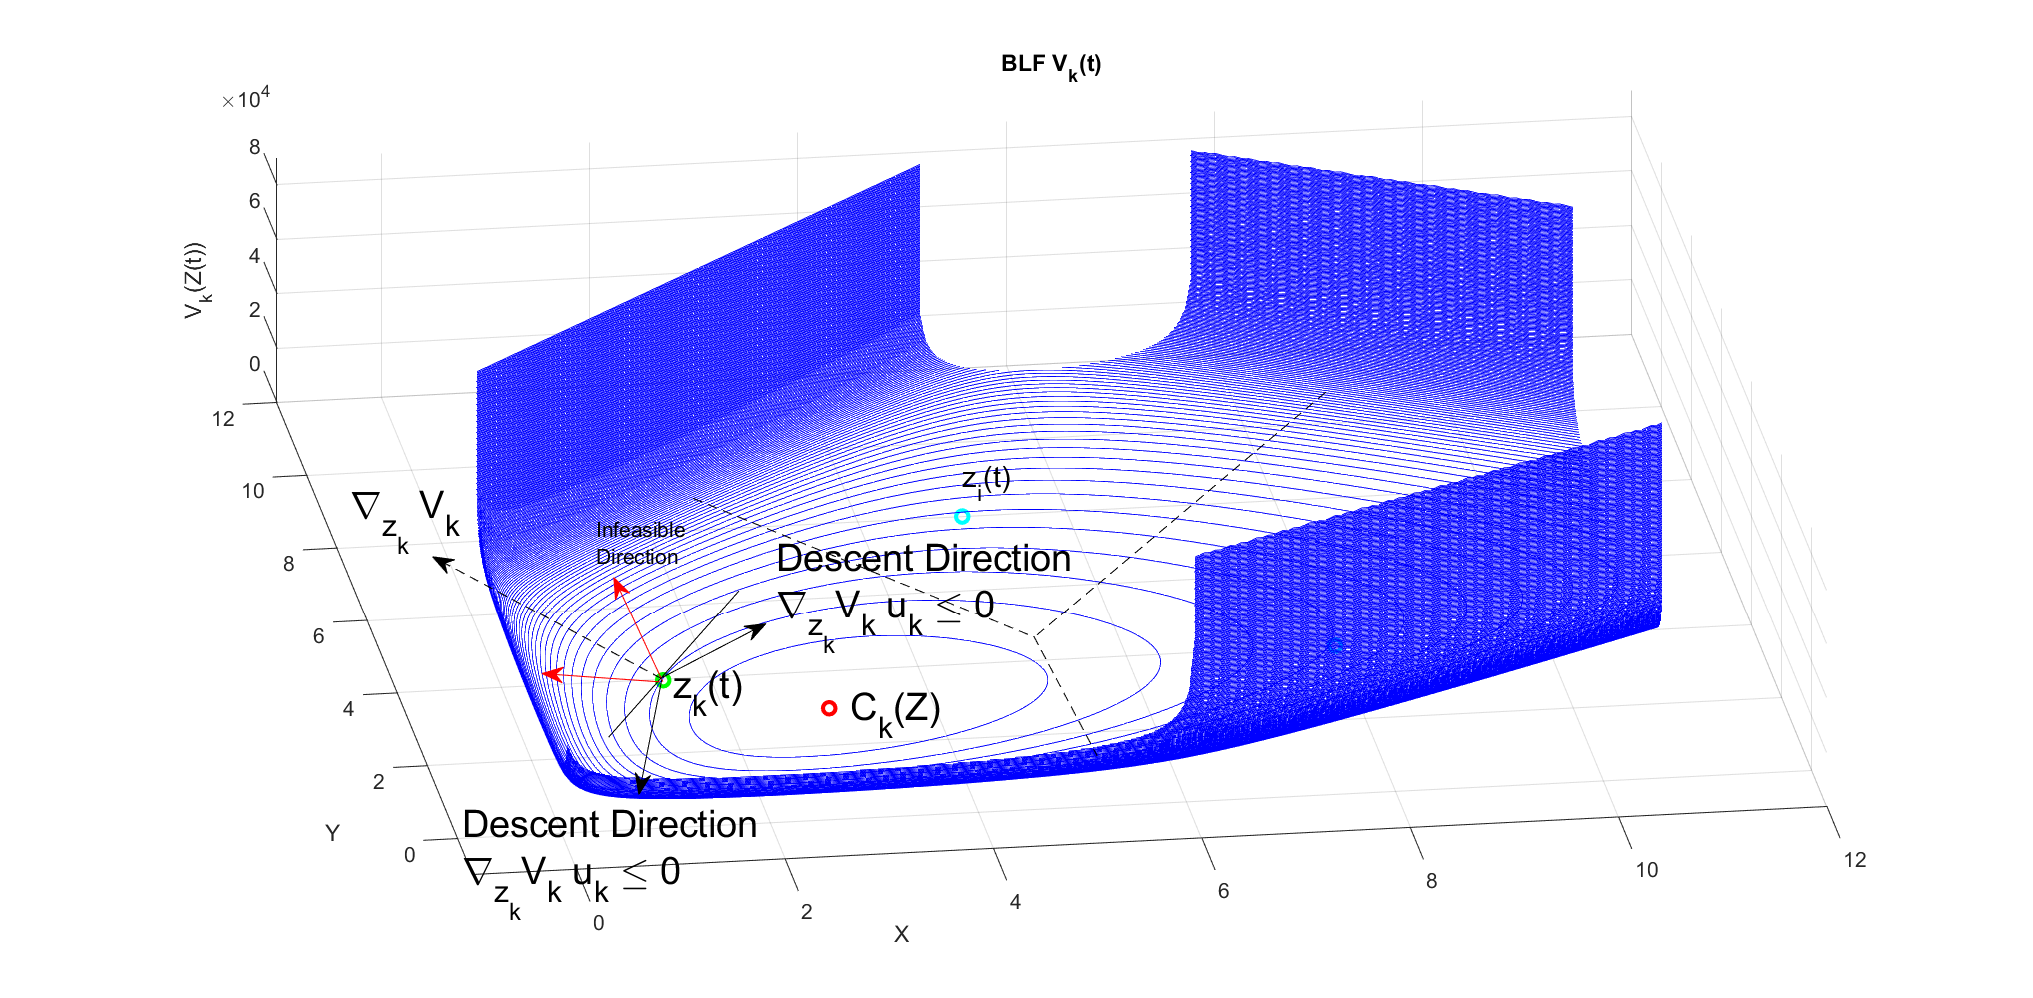
\includegraphics[width=1\linewidth]{BLF_3D_Contour_zoom}
	\caption{Barrier Lyapunov Function and The Feasible Direction of Agent $k$}
	\label{fig:Contour_3D}
\end{figure}

\noindent Figure \ref{fig:Contour_3D} demonstrates the concept of Proposition 2, there exists a feasible movement that ensures the state constraint. \\

\noindent \textbf{Proof.} \\
From the initial condition, agent $k$ and the center of Voronoi partition $C_k$ is inside the coverage region so the BLF is well defined. Because the proposed function is differentiable, the directional derivative delivers a descent and ascent direction of $V_k{Z}$ related to the variable $z_k$. Since the region $\interior Q$ is convex and the BLF is designed so that it always has a local optimum at $C_k$, it implies that $z_k$ is feasible if it follows the descent direction.

\noindent Due to the complexity of this problem, we must analyze all of the necessary and sufficient conditions to ensure the feasibility for all agents. This will be presented with more details in the Discussion in chapter 5. \\

\noindent According to the proposition 2, we analyze $\frac{\partial V_k(Z)}{dz_k}\dot z_k$ to obtain a control law for agent $k$

\begin{equation} \notag
\begin{split}
%V_k(Z) & = \displaystyle\sum_{j=1}^{m} [ln(\frac{b_j - a_{jx}C_{kx} - a_{jy}C_{ky}}{b_j - a_{jx}z_{kx} - a_{jy}z_{ky}})]^2 \\
& \frac{\partial V_k(Z)}{dz_k}\dot z_k \\
& = \frac{\partial V_k(Z)}{dz_{kx}}\dot z_{kx} + \frac{\partial V_k(Z)}{dz_{ky}}\dot z_{ky} \\
& = \dot z_{kx} \displaystyle\sum_{j=1}^{m} \frac{\partial}{\partial z_{kx}} [ln(\frac{b_j - a_{jx}C_{kx} - a_{jy}C_{ky}}{b_j - a_{jx}z_{kx} - a_{jy}z_{ky}})]^2 + \dot z_{ky} \displaystyle\sum_{j=1}^{m} \frac{\partial}{\partial z_{ky}} [ln(\frac{b_j - a_{jx}C_{kx} - a_{jy}C_{ky}}{b_j - a_{jx}z_{kx} - a_{jy}z_{ky}})]^2 \\
%
& = \displaystyle\sum_{j=1}^{m} 2ln(\frac{b_j - a_{jx}C_{kx} - a_{jy}C_{ky}(t)}{b_j - a_{jx}z_{kx} - a_{jy}z_{ky}})(\frac{-a_{jx}\frac{\partial C_{kx}}{\partial z_{kx}}\dot z_{kx} - a_{jy}\frac{\partial C_{ky}}{\partial z_{kx}}\dot z_{ky}}{b_j - a_{jx}C_{kx} - a_{jy}C_{ky}} + \frac{-a_{jx}\dot z_{kx} - a_{jy}\dot z_{ky}\dot z_{ky}}{b_j - a_{jx}z_{kx} - a_{jy}z_{ky}}) \\ 
\end{split}
\end{equation}

\noindent Substitute the partial derivative of virtual mass ${z_k}$ from (\ref{vm_derivatve}) into ${\dot V(Z)}$, we obtain
\begin{equation} \notag
\begin{split}
&\frac{\partial V_k(Z)}{dz_k}\dot z_k = -\mu_k(\psi_{k})\frac{v_k}{\norm{w_{k_0}}}. \\
&\underbrace{cos(\psi_{k}) \displaystyle\sum_{j=1}^{m} 2ln(\frac{b_j - a_{jx}C_{kx} - a_{jy}C_{ky}}{b_j - a_{jx}z_{kx} - a_{jy}z_{ky}})(\frac{a_{jx}cos(\theta_{k}) + a_{jy}sin(\theta_{k})}{b_j - a_{jx}z_{kx} - a_{jy}z_{ky}} - \frac{a_{jx}\frac{\partial C_{kx}}{\partial z_{kx}}cos(\theta_{k}) + a_{jy}\frac{\partial C_{ky}}{\partial z_{kx}}sin(\theta_{k})}{b_j - a_{jx}C_{kx} - a_{jy}C_{ky}})}_{M_k(t)}
\end{split}
\end{equation}

\noindent The complicated $M_k(t)$ can be obtained by the full state feedback at time t, which are ${z_k(t), \theta_{k}(t), C_k(t)}$ and constant $A \txtspc{,} b$. Note that the gradient $ [\frac{\partial C_{kx}}{\partial z_{kx}} \txtspc{ } \frac{\partial C_{ky}}{\partial z_{ky}}] $ is complicated but there already exists an analytical formulation. These terms will be introduced later in the controller design section. We obtain
\begin{equation} \label{time_derivative_BLF}
\begin{split}
\frac{\partial V_k(Z)}{dz_k} &  = -\mu_k(t)\frac{v_k}{\norm{w_{k_0}}} M_k(t)\\
\end{split}
\end{equation}

\noindent \textbf{Intuitive Explanation of the Switching Control Law:} \\
Note that we have two Lyapunov functions in our derivation, which are ${H(Z(t))}$ and ${V(Z(t))}$. While the negative time derivative of $H(Z(t))$ ensures the asymptotic stability of the coverage control, it does not reflect the feasibility of the state. On the other hand, from proposition 2, there exist a feasible movement of agent $z_k$, but does not guarantee asymptotic stability of coverage control because its time derivative is not always non-positive. \\
The idea behind is to use the property of Proposition 2 that whenever $\frac{\partial V_k(Z)}{dz_k}\dot z_k \leq 0$, ${z_k \in \interior{Q}}$, the virtual mass ${z_k}$ is allowed to move. As long as there exists a control input with a positive control gain ${\mu_k}$ that satisfies this condition, it is shown that ${\dot H(Z(t)) < 0}$ and the coverage control converge asymptotically. \\
Additionally, ${\mu_k \in \mathbb{R}_+}$ must satisfy the condition obtained from section 3.2 to handle the input saturation. \\
\textbf{Proposition 3:} \\
The following switching condition ensures that all agents' virtual mass always stay inside the interior of region Q and asymptotically converge to the set of centroidal Voronoi configuration. \\ 
\begin{equation} \label{switching_law}
\begin{split} 
\mu_k(t) = \twopartdef {\mu_k(t) \in \mathbb{R}_+} {, M_k(t) \geq 0} {0} {, M_k(t) < 0}
\end{split}
\end{equation}
\noindent \textbf{Proof.} \\
$\bullet$ \textbf{\textit{Feasibility of States}} \\
\noindent \underline{${M_k(t) \geq 0 \implies \mu_k(t) \in \mathbb{R}_+}$} \\
\begin{equation} \notag
\begin{split} 
\frac{\partial V_k(Z)}{dz_k} & = -\mu_k(t)\frac{v_k}{\norm{w_{k_0}}} M_k(t) \\
& = -\norm{\mu_k(t)}\frac{v_k}{\norm{w_{k_0}}} \norm{M_k(t)} \leq 0 \\
\text{Proposition 2} \implies & z_k(t) \in \interior Q \txtspc{as} t \rightarrow \infty 
\end{split}
\end{equation}

\noindent \underline{${M_k(t) < 0  \implies \mu_k(t) = 0}$} 
\[\exists t \in [t_0 \txtspc{ } \infty) \txtspc{ } z_k(t) \in \interior{Q}\]
\[\mu_k(t) = 0 \implies \dot z_k(t) = 0 \implies z_k(t + \delta t) = z_k(t) \in \interior{Q} \txtspc{ } for \txtspc{ } \delta t \rightarrow 0\]
Intuitively, if the virtual mass of an agent is not allowed to move due to state feasibility, the control input forces it to stay there by keep the agent rotate at the current virtual mass. \\

\noindent (\ref{switching_law}) fulfills state constraints (q.e.d). \\

\noindent $\bullet$ \textbf{\textit{Asymptotic Convergence of Virtual Masses on Centroidal Voronoi Configuration}} \\
\noindent \underline{${M_k(t) \geq 0 \implies \mu_k(t) \in \mathbb{R}_+}$} \\
\[\mu_k(t) \in \mathbb{R}_+ \implies \dot H(Z) = - \displaystyle\sum_{k=1}^{n} \frac{\mu_k(\psi_{k})M_{V_{k}}v_{k}}{\norm{w_{0}}\norm{z_{k} - C_{V_{k}}}} \langle{z_{k} - C_{V_{k}},e^{i\theta_{k}}}\rangle^{2} \leq 0\] 
From Proposition 1: LaSalle' invariance principle implies that system approaches the unique stable equilibrium points if and only if ${z_{k} = C_{V_{k}} \forall k \in \{1,...,n\}}$ \\

\noindent \underline{${M_k(t) < 0  \implies \mu_k(t) = 0}$} \\
Assume model's dynamic approaches the set of stable equilibrium points at time ${t \in [t_0 \txtspc{ } \infty)}$ \\
This set is defined as ${\Omega = \{Z \in \interior Q| \dot H(Z(t')) = 0 \txtspc{ } \forall t' \in [t \txtspc{ } \infty)\}}$. We have
\[\dot H(Z(t')) = 0 \txtspc{ } \forall t' \in [t \txtspc{ } \infty)\]
\[\Leftrightarrow \mu_k(t') = 0 \txtspc{ } \forall k \in \{1,...,n\} \txtspc{ } \forall t' \in [t \txtspc{ } \infty) \]
\[\Leftrightarrow M_k(t') < 0 \txtspc{ } \forall k \in \{1,...,n\} \txtspc{ } \forall t' \in [t \txtspc{ } \infty) \tag{P3.1} \] 

\noindent If every agent rotates around its unchanged virtual mass, the center of each Voronoi cell remains constant \\
\[\mu_k(t') = 0 \implies \dot z_k(t') = 0 \implies z_k(t') = z_k(t) \txtspc{ } \forall k \in \{1,...,n\} \txtspc{ } \forall t' \in [t \txtspc{ } \infty)\]
\[\implies C_k(t') = C_k(t) = const  \txtspc{ } \forall k \in \{1,...,n\} \txtspc{ } \forall t' \in [t \txtspc{ } \infty)\]

\noindent Then from the definition, $\psi_{k}$ has the same dynamic with ${\theta_{k}}$\\
\[\mu_k(t') = 0 \implies u_{k}(t') = w_{k_0} \txtspc{ } \text{from (\ref{control_with_consraint})} \txtspc{ } \forall t' \in [t \txtspc{ } \infty)\]
\[\psi_{k} = \angle (z_{k} - C_{V_{k}}, v_{k}e^{i\theta_{k}}) \txtspc{,} C_k(t') = const \txtspc{,} \dot z_k(t) = 0 \implies \dot \psi_{k} = \dot \theta_{k} = w_{k_0}\]

\noindent It is shown that if these equilibrium points are not the CVT by the following contradiction
\[\dot \psi_{k} = w_{k_0} \implies \exists t' \in [t \txtspc{ } \infty): cos(\psi_{k}(t')) = 0 \]
\[\implies \exists t' \in [t \txtspc{ } \infty): M_k(t') = 0\]

\noindent This contradicts the statement (P3.1) and consequently these equilibrium points are unstable. Only when the virtual masses of every agent coincide the set of centroidal Voronoi configuration, ${H(Z) = 0 \txtspc{,} \dot H(Z) = 0}$. The theorem of Barbashin states that the system is asymptotic stable. (q.e.d)

\section{Controller Design}
\subsection{Scaling Factor for Input Saturation}
In \textbf{Proposition 1} (Subsection 3.2. Problem of Input Constraints) we pointed out the existence of an feasible positive control gain ${\mu_k(\psi_{k})}$. The following derivation determines ${\mu_k(\psi_{k}): [0 \txtspc{ } 2\pi] \rightarrow \mathbb{R}_+}$ in detail. \\
% PROBLEM STATEMENT **************************************************************************************************************************************************
$\bullet$ \textbf{Problem statement}\\
For a given reference ${C_{V_{k}} = [C_{kx} \txtspc{ } C_{ky}]^{T} \in \mathbb{R}^{2}}$, upper and lower input saturation ${U_{up}, U_{low} > 0}$, desired orbiting velocity ${w_{k_0}\in [-U_{low} \txtspc{ } U_{up}]}$. From the measurement of virtual mass's current position ${z_{k} = [z_{kx} \txtspc{ } z_{ky}]^{T} \in \mathbb{R}^{2}}$ and heading orientation  ${\theta_{k} \in [0, 2\pi]}$. By defining ${\psi_{k} = \angle (z_{k} - C_{V_{k}}, v_{k}e^{i\theta_{k}}) \in [0 \txtspc{ } 2\pi]}$, find ${\mu_k(\psi_{k}): [0 \txtspc{ } 2\pi] \rightarrow \mathbb{R}_+}$ to keep the control input ${u_{k} = w_{k_0} + \mu_k(\psi_{k})sign(w_{k_0})cos(\psi_{k})}$ always stay in feasible region, which means ${u_{k} \in [-U_{low} \txtspc{ } U_{up}]}$. \\
Task: Find
\begin{equation} \notag
\begin{split}
&\mu_k(\psi_{k}) \in \mathbb{R}_+ \txtspc{,} \forall \psi_{k} \in [0 \txtspc{ } 2\pi]\\
\end{split}
\end{equation}
so that 
\begin{equation}
\begin{split}
& u_{k} = w_{k_0} + \mu_{k}(\psi_{k})sign(w_{k_0})cos(\psi_{k}) \\
& u_k \in [-U_{low} \txtspc{ } U_{up}] \txtspc{,} \forall \psi_{k} \in [0 \txtspc{ } 2\pi] \\
\end{split}
\end{equation}
% SOLUTION **************************************************************************************************************************************************
\noindent $\bullet$ \textbf{Solution} \\
\noindent For any ${C_{V_{k}}}$, a desired orbiting angular velocity is ${w_{k_0}}$ known in advance. From these factors, we propose a control gain that depends from actual ${\psi_{k}}$ and ${w_{k_0}}$ as following \\

\indent $\blacksquare$ If ${w_{k_0} > 0}$ 
\begin{equation} \label{adaptive_gain_positive_w0} %***************************************************
\begin{split}
& \mu_k(\psi_{k})sign(w_{k_0}) \\
& = \mu_k(\psi_{k})\\
& = \twopartdef {k_1 \in \mathbb{R} \txtspc{,} 0 < k_1 \leq U_{up} - \norm{w_{k_0}}} 		{for ${ }$ \psi_{k} \in [\frac{\pi}{2} \txtspc{ } \frac{3\pi}{2}]} 
				{k_2 \in \mathbb{R} \txtspc{,} 0 < k_2 \leq U_{low} + \norm{w_{k_0}}} 		{for ${ }$ \psi_{k} \in [0 \txtspc{ } \frac{\pi}{2}] \cup [\frac{3\pi}{2} \txtspc{ } 2\pi]} \\
\end{split}
\end{equation}
%
\indent $\blacksquare$ If ${w_{k_0} < 0}$ 
\begin{equation} \label{adaptive_gain_negative_w0} %***************************************************
\begin{split}
& \mu_k(\psi_{k})sign(w_{k_0}) \\
& = -\mu_k(\psi_{k})\\
& = \twopartdef {-k_1 \in \mathbb{R} \txtspc{,} 0 < k_1 \leq U_{low} - \norm{w_{k_0}}} 		{for ${ }$ \psi_{k} \in [\frac{\pi}{2}\txtspc{ } \frac{3\pi}{2}]} 
				{-k_2 \in \mathbb{R} \txtspc{,} 0 < k_2 \leq U_{up} + \norm{w_{k_0}}}			{for ${ }$ \psi_{k} \in [0\txtspc{ } \frac{\pi}{2}] \cup [\frac{3\pi}{2}\txtspc{ } 2\pi]} \\
\end{split}
\end{equation}

% SOLUTION **************************************************************************************************************************************************
\noindent $\bullet$ \textbf{Proof.} The feasibility of control input\\
\indent $\blacksquare$ For predefined ${w_{k_0} > 0}$ 
\begin{equation} \notag %\label{Proof_positive_adaptive_gain} %***************************************************
\begin{split}
u_{k} & = w_{k_0} + \mu_k(\psi_{k})sign(w_{k_0})cos(\psi_{k})\\
& = \norm{w_{k_0}} + \mu_k(\psi_{k})cos(\psi_{k})  \\
(\ref*{adaptive_gain_positive_w0}) \implies & \twopartdef {u_{k} = \norm{w_{k_0}} + k_1cos(\psi_{k})} {for \txtspc{ } 0 < k_1 \leq U_{up} - \norm{w_{k_0}} \txtspc{,}\psi_{k} \in [\frac{\pi}{2}  \txtspc{ } \frac{3\pi}{2}]}
{u_{k} = \norm{w_{k_0}} + k_2cos(\psi_{k})} {for \txtspc{ } 0 < k_2 \leq U_{low} + \norm{w_{k_0}} \txtspc{,} \psi_{k} \in [0 \txtspc{ } \frac{\pi}{2}] \cup [\frac{3\pi}{2}\txtspc{ } 2\pi]}\\
\implies & \twopartdef {u_{k} \leq \norm{w_{k_0}} + (U_{up} -\norm{w_{k_0}})} {for ${ }$ \psi_{k} \in [\frac{\pi}{2} \txtspc{ } \frac{3\pi}{2}]} {u_{k} \geq \norm{w_{k_0}} + (U_{low} + \norm{w_{k_0}})}   {for ${ }$ \psi_{k} \in [0 \txtspc{ } \frac{\pi}{2}] \cup [\frac{3\pi}{2} \txtspc{ } 2\pi]} \\
\implies & u_{k} \in [-U_{low} \txtspc{ } U_{up}] \txtspc{ } \forall \psi_{k} \in [0 \txtspc{ } 2\pi] (q.e.d) \\
\end{split}
\end{equation}

\indent $\blacksquare$ Analog for ${w_{k_0} < 0}$ 
\begin{equation} \notag %\label{Proof_positive_adaptive_gain} %***************************************************
\begin{split}
u_{k} & = w_{k_0} + \mu_k(\psi_{k})sign(w_{k_0})cos(\psi_{k})\\
& = -\norm{w_{k_0}} - \mu_k(\psi_{k})cos(\psi_{k})  \\
(\ref*{adaptive_gain_negative_w0}) \implies & \twopartdef {u_{k} = -\norm{w_{k_0}} - k_1cos(\psi_{k})} {for \txtspc{ } 0 < k_1 \leq U_{low} - \norm{w_{k_0}} \txtspc{,}\psi_{k} \in [\frac{\pi}{2}  \txtspc{ } \frac{3\pi}{2}]} 
{u_{k} = -\norm{w_{k_0}} - k_2cos(\psi_{k})} {for \txtspc{ } 0 < k_2 \leq U_{up} + \norm{w_{k_0}} \txtspc{,} \psi_{k} \in [0 \txtspc{ } \frac{\pi}{2}] \cup [\frac{3\pi}{2}\txtspc{ } 2\pi]}\\
\implies & \twopartdef {u_{k} \geq -\norm{w_{k_0}} - (U_{low} -\norm{w_{k_0}})} {for ${ }$ \psi_{k} \in [\frac{\pi}{2} \txtspc{ } \frac{3\pi}{2}]} {u_{k} \leq -\norm{w_{k_0}} + (U_{up} + \norm{w_{k_0}})}   {for ${ }$ \psi_{k} \in [0 \txtspc{ } \frac{\pi}{2}] \cup [\frac{3\pi}{2} \txtspc{ } 2\pi]} \\
\implies & u_{k} \in [-U_{low} \txtspc{ } U_{up}] \txtspc{ } \forall \psi_{k} \in [0 \txtspc{ } 2\pi] (q.e.d) \\
\end{split}
\end{equation}

\subsection{Model Based Control Design for State Constraint}
Recall
\begin{equation} \label{M_k}
\begin{split}
M_k(t) = & cos(\psi_{k}) \displaystyle\sum_{j=1}^{m} 2ln(\frac{b_j - a_{jx}C_{kx} - a_{jy}C_{ky}}{b_j - a_{jx}z_{kx} - a_{jy}z_{ky}})\\
& \txtspc{    } (\frac{a_{jx}cos(\theta_{k}) + a_{jy}sin(\theta_{k})}{b_j - a_{jx}z_{kx} - a_{jy}z_{ky}} - \frac{a_{jx}\frac{\partial C_{kx}}{\partial z_{kx}}cos(\theta_{k}) + a_{jy}\frac{\partial C_{ky}}{\partial z_{kx}}sin(\theta_{k})}{b_j - a_{jx}C_{kx} - a_{jy}C_{ky}})
\end{split}
\end{equation}
The switching controller law from (\ref{switching_law}) is used to consider whether each agent moves or rotates around its virtual mass through the control gain as follows 
\[\mu_k(t) = \twopartdef {\mu_k(t) \in \mathbb{R}_+} {M_k(t) \geq 0} {0} {M_k(t) < 0}\]

\noindent In [5], Appendix A, Lee already formulated the gradient of $C_k = [\frac{\partial C_{kx}}{\partial z_{kx}} \txtspc{ } \frac{\partial C_{ky}}{\partial z_{ky}}]$ as \\
\begin{equation} \label{grad_C}
\frac{\partial {C}^{(a)}_k}{\partial {z}^{(b)}_k} = \frac{(\int_{\partial V_{i,j}}^{} \phi(q)q^{(a)} \frac{q^{(b)} - {z}^{(b)}_k}{\norm{z_j - z_i}} dq)}{m_k} - \frac{(\int_{\partial V_{i,j}}^{} \phi(q)\frac{q^{(b)} - {z_k}^{(b)}}{\norm{z_j - z_i}} dq)(\int_{V_k(Z)}^{} \phi(q)q^{(a)}dq)}{m^2_k}
\end{equation}
where $a,b \in {x,y}$ and $m_k = \int_{V_k(Z)}^{} \phi(q)dq$. \\
With all of the necessary state feedback, the implementation of a controller for ${k-th}$ agent is presented as follows

\begin{algorithm} [H] % enter the algorithm environment
	\caption{Computation of Control Input for n agents} % give the algorithm a caption
	\label{alg1} % and a label for \ref{} commands later in the document
	\textbf{Data:}\\
	- Information of dominating region ${Q}$: ${A \in \mathbb{R}^{m \times 2} \txtspc{,} b \in \mathbb{R}^m }$. \\
	- Input limits: ${[-U_{k_{low}} \txtspc{ } U_{k_{up}}] \txtspc{,} \forall k \txtspc{,} U_{k_{low}},U_{k_{up}} > 0}$ \\
	- Desired orbiting velocity: ${w_{k_0} \in [-U_{k_{low}} \txtspc{ } U_{k_{up}}]}$ \\
	- Constant heading velocity: ${v_k \in \mathbb{R}_+}$ \\
	\textbf{Result:} \\
	- Control input for each agent: ${u_k}$ \\
	\noindent\rule{\textwidth}{1pt}

	$\bullet$ \textbf{Initialization} \\% // Do once \\
	- Choose feasible control gain: (\ref{adaptive_gain_positive_w0}),(\ref{adaptive_gain_negative_w0}) ${\implies}$  ${\mu_k \in \{k_1,k_2\} \txtspc{ } \forall{k} \in \{1,...,n\}}$ \\
	- Initialize all agents position that satisfy: ${z_k(t_0) \in \interior{Q} \txtspc{ } \forall{k} \in \{1,...,n\}}$ \\
	
	$\bullet$ \textbf{Loop}% // Execution
	\begin{algorithmic} % enter the algorithmic environment
	\FOR{k = 1 \TO n } 
		\STATE { } 
		\STATE {${\psi_{k} \leftarrow arccos(\frac{\langle{z_{k} - C_{V_{k}}},{e^{i\theta_{k}}}\rangle}{\norm{z_{k} - C_{V_{k}}}})}$} 
		\STATE { } 
		\IF{${\psi_{k} \in [\frac{\pi}{2} \txtspc{ } \frac{3\pi}{2}]}$} 
			\STATE {${\mu_k \leftarrow k_1}$} 
		\ELSE 
			\STATE {${\mu_k \leftarrow k_2}$} 
		\ENDIF
		\STATE { } 

		\STATE {${(\frac{\partial C_{kx}}{\partial z_{kx}} \txtspc{  } \frac{\partial C_{ky}}{\partial z_{ky}}) \leftarrow (\ref{grad_C})}$} 
		\STATE { } 
		
		\STATE {${M_k  \leftarrow (\ref{M_k})}$} 
	
		\IF{${M_k \geq 0}$} 
			\STATE {${\mu_k \leftarrow \mu_k}$} 
		\ELSE 
			\STATE {${\mu_k \leftarrow 0}$} 
		\ENDIF
		
		\STATE { } 

		\STATE {${u_k \leftarrow w_{k_0} + \mu_k sign(w_{k_0})cos(\psi_{k})}$} 
	\ENDFOR	
	\end{algorithmic} % enter the algorithmic environment	
	\textbf{Return:} ${u_k \txtspc{ } \forall k \in \{1,...,n\}}$\\
\end{algorithm}





\chapter{Evaluation}

In order to evaluate the proposed control method, we create the simulation platform using MATLAB and VREP (Coppelia Sim). The problem configuration is a group of five unicycle-type agents cover a convex bounded region with a constant heading velocity. They are not allowed to get out of the region during the operation and the rotation velocity is limited. Figure \ref{fig:VREP} depicts the scenario of this coverage problem. 
\begin{figure} [h]
	\centering
	\includegraphics[width=1\linewidth]{VREP_SIM}
	\caption{5 Agents - Convex region}
	\label{fig:VREP}
\end{figure}

During the operation, all data of agents are logged for the evaluation. Data such as virtual mass's position and control input, are plotted intuitively. Figure \ref{fig:VREP_state} demonstrates the trajectories of five agents created throughout the operation. They never cross the boundary lines, this implies the state constraint is not violated. \\
\begin{figure} [!h]
	\centering
	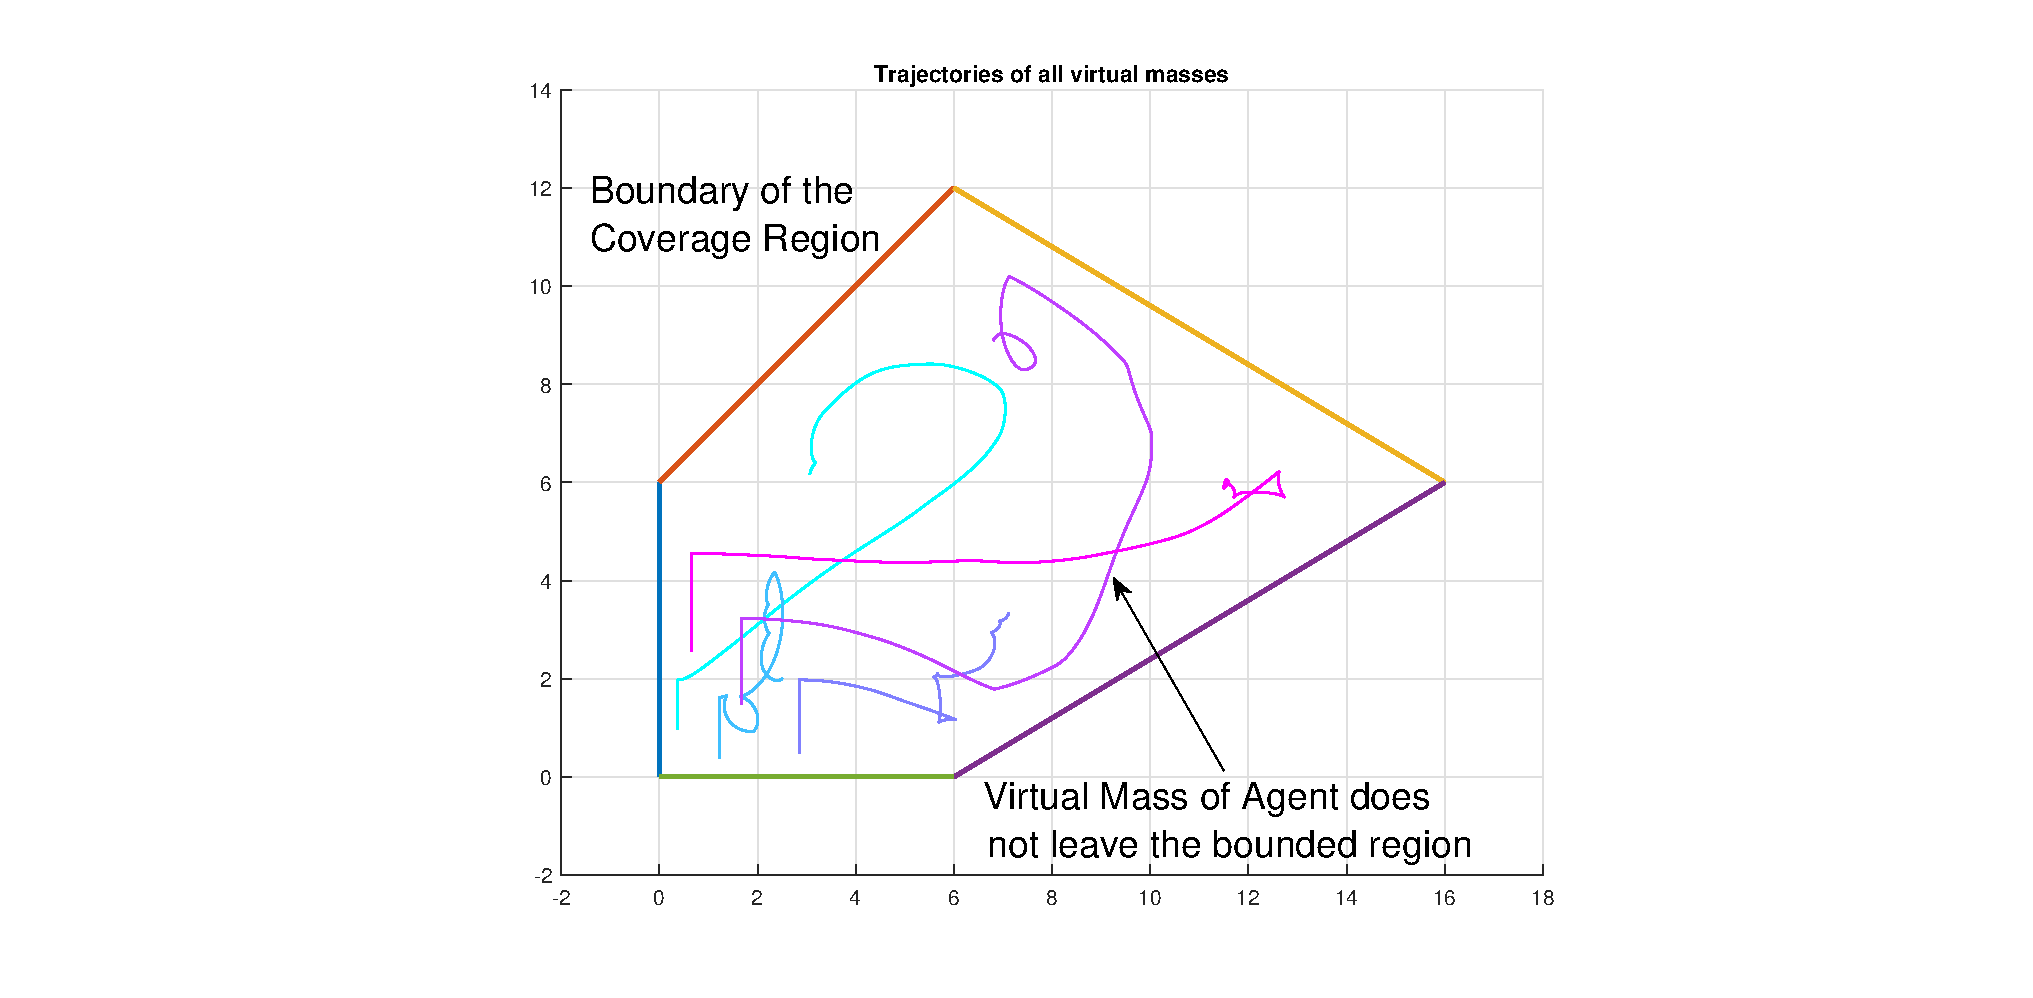
\includegraphics[width=1.3\linewidth]{Eva_VREP_trajectories}
	\caption{Feasibility of States}
	\label{fig:VREP_state}
\end{figure}

\begin{figure} [!h]
	\centering
	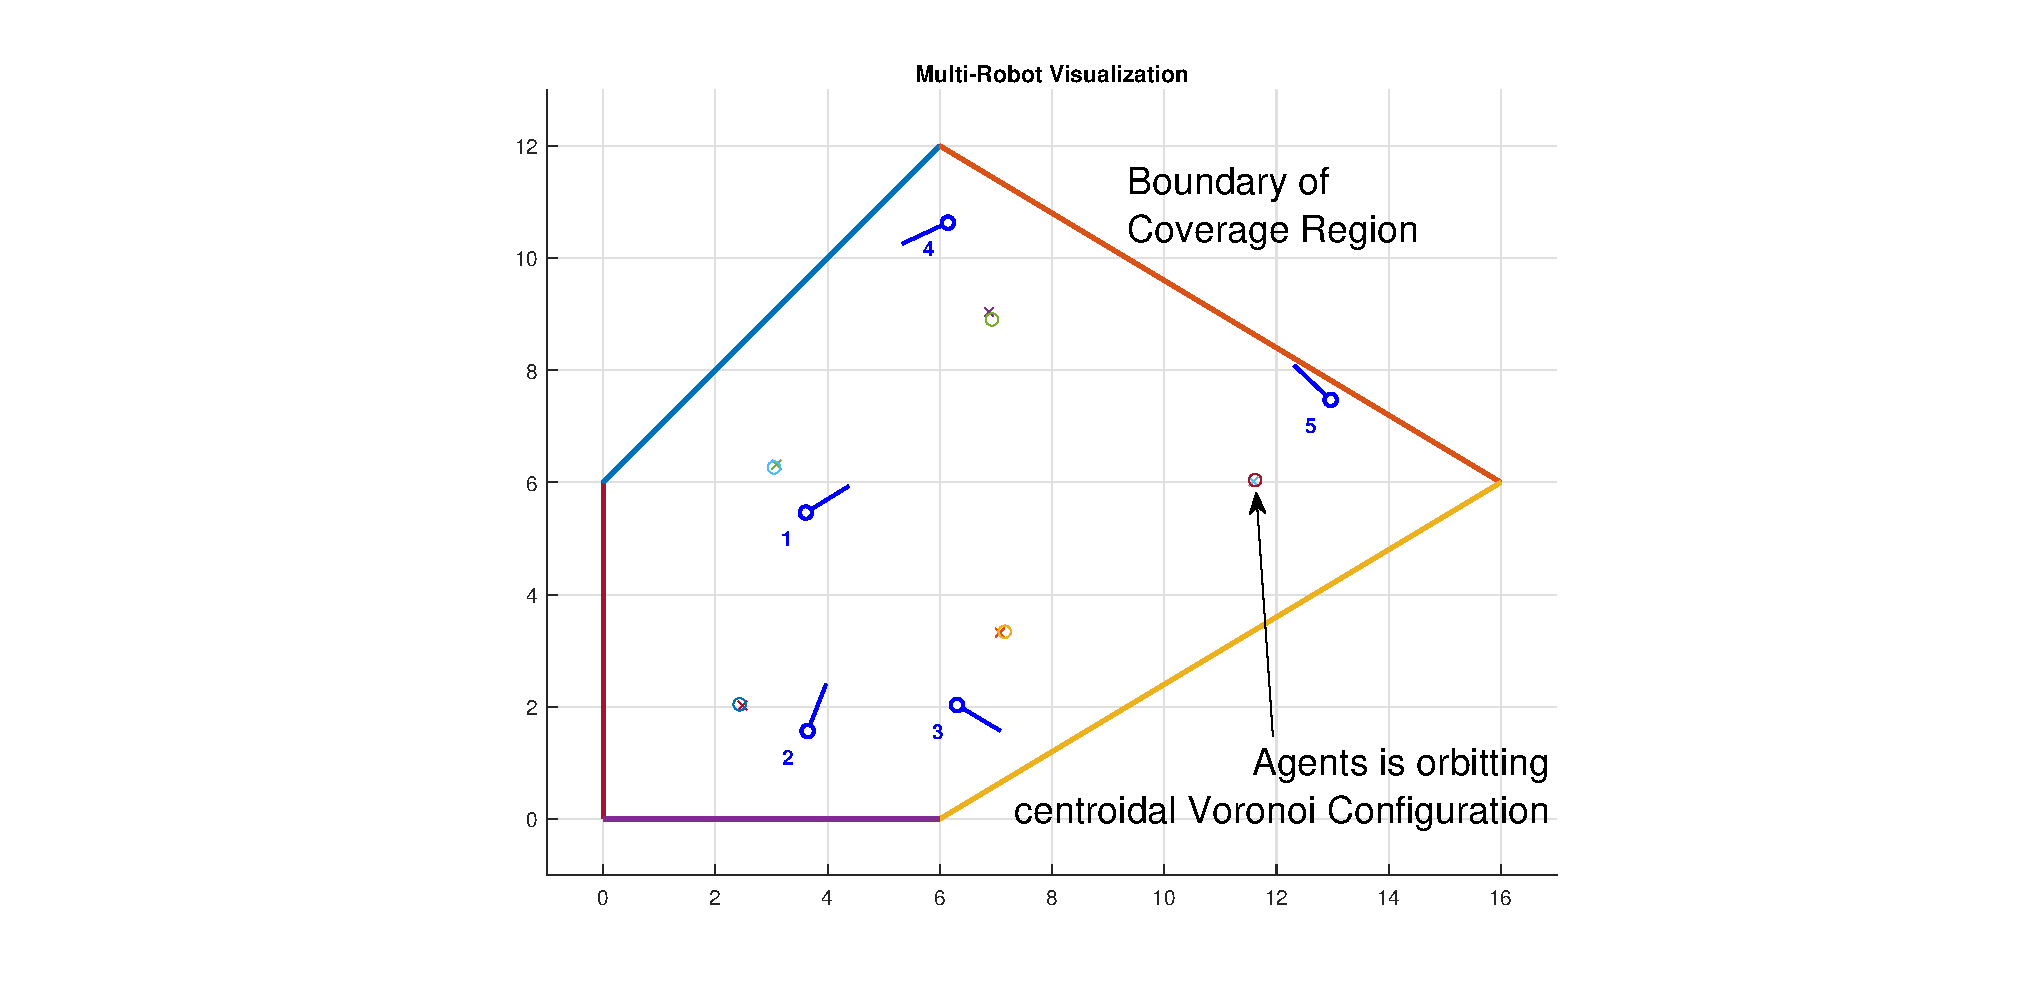
\includegraphics[width=1.3\linewidth]{Eva_VREP_bot_final}
	\caption{Final State of the Coverage Control}
	\label{fig:VREP_bot_final}
\end{figure}
Figure \ref{fig:VREP_bot_final} and \ref{fig:VREP_voronoi} depicts the final state of the coverage problem. It can be seen that all agents are orbiting their virtual masses, which converge to the set of centroidal Voronoi configuration. \\
\begin{figure} [!h]
	\centering
	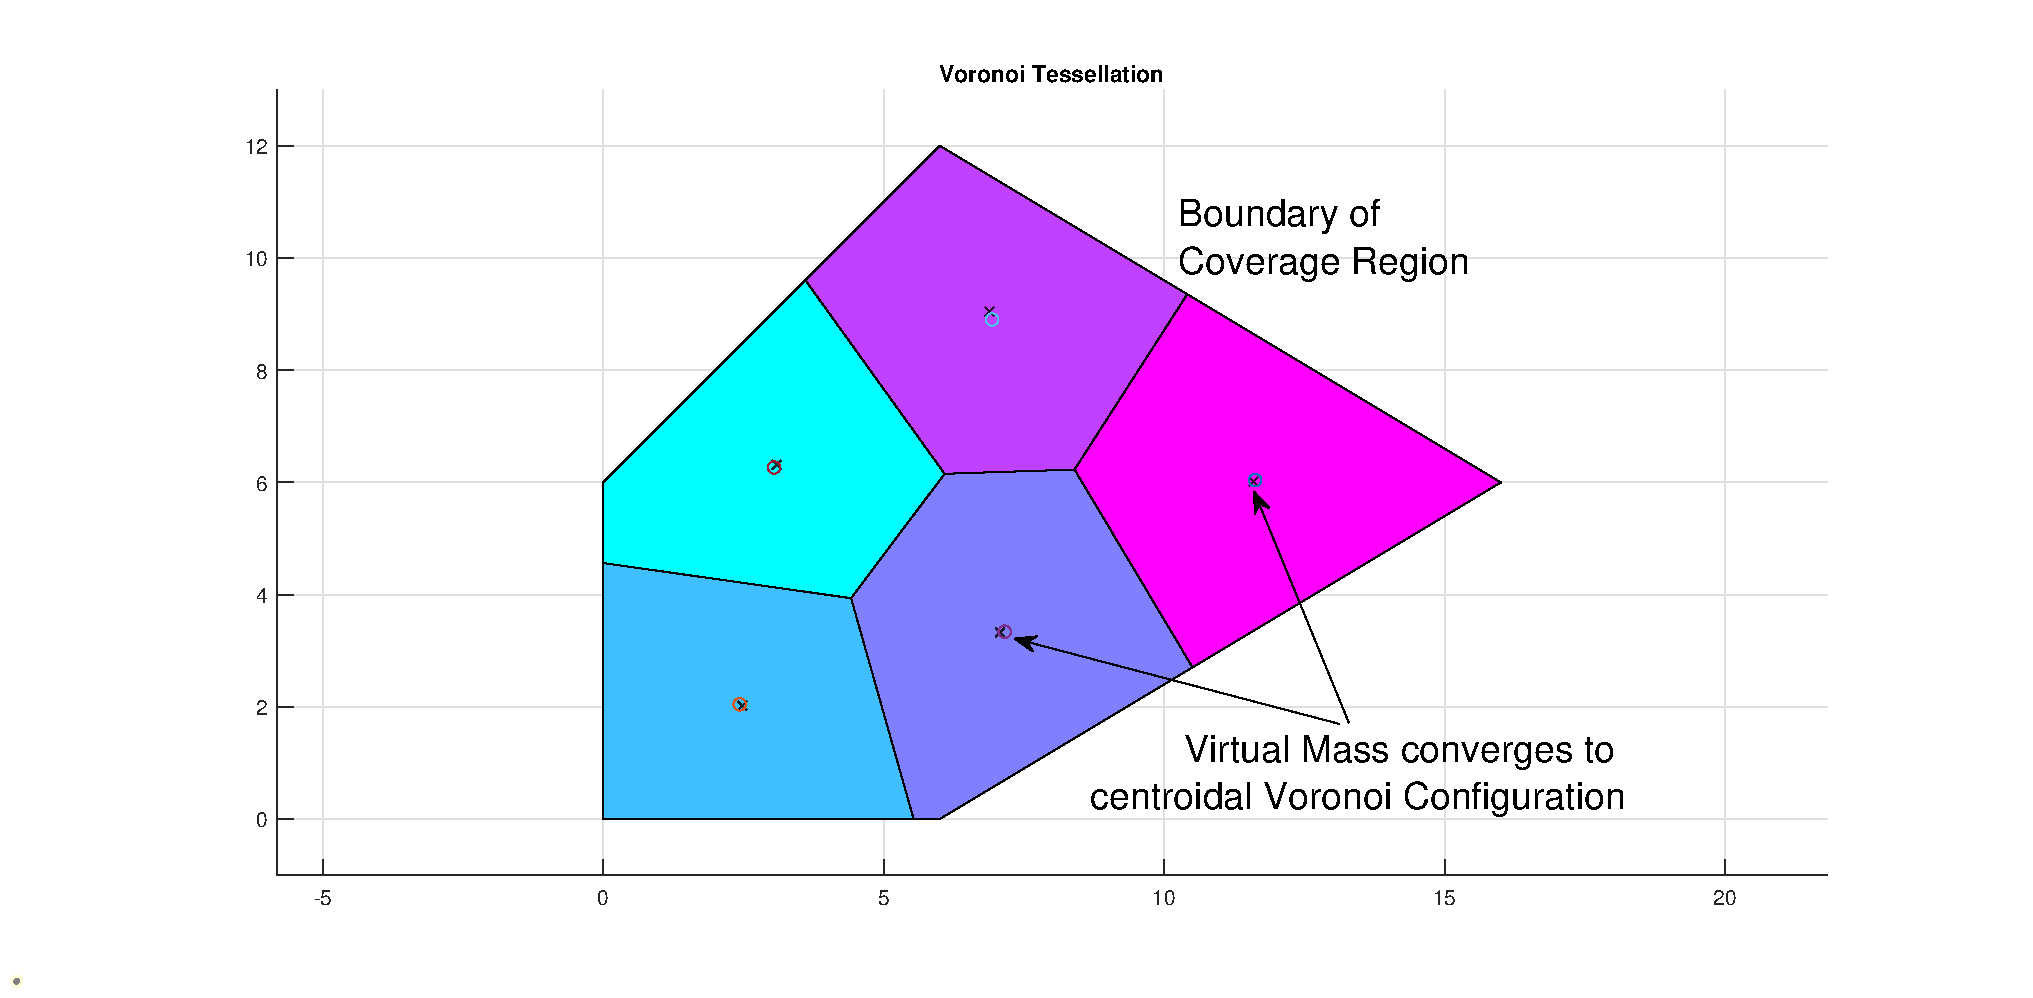
\includegraphics[width=1\linewidth]{Eva_VREP_Voronoi}
	\caption{Agents Orbit the Centroidal Voronoi Configuration}
	\label{fig:VREP_voronoi}
\end{figure}

The maximal rotation velocity of agents are configured to be -0.5 rad/s and 0.5 rad/s. As can be seen in Figure \ref{fig:VREP_control_input} that the control input is always inside the red bounded lines, this indicates that the input constraint are never violated. \\
\begin{figure} [!h]
	\centering
	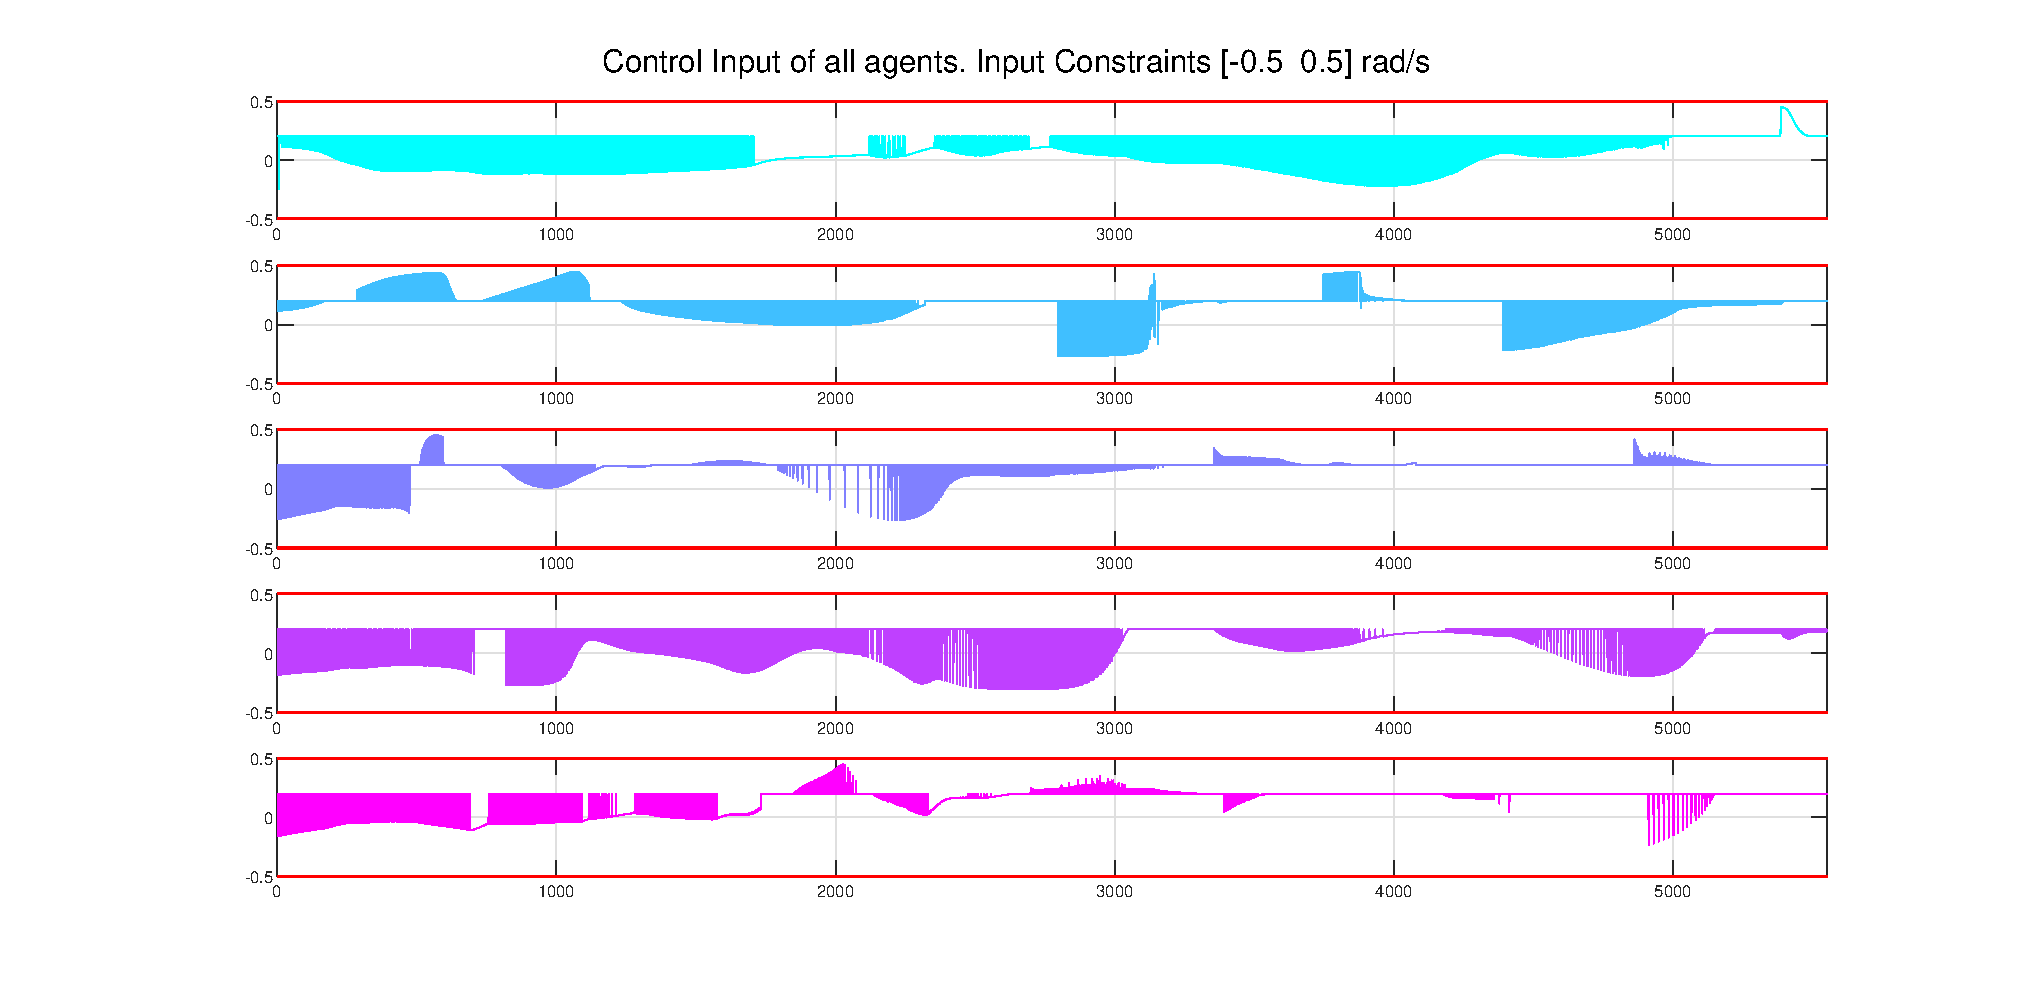
\includegraphics[width=1\linewidth]{Eva_VREP_control_input}
	\caption{Feasible Control Input}
	\label{fig:VREP_control_input}
\end{figure}

Using this simulation environment, we also evaluate the coverage problem with different convex regions such as triangle or rectangle form. The results depicts the reliability and feasibility of the proposed control method.
\chapter{Discussion}
In the analysis of the state constraint, we introduce a Barrier Lyapunov Function and use the proposition 2 to show the feasibility of agent $z_k$. However, this method is yet still not proven under a mathematical analysis. There might be some sufficient and necessary conditions that must be fulfilled. In this chapter, we discuss about this challenge with more details and propose related future work in the conclusion. \\ \\
%\section{Problem Review}
\noindent We introduce the coverage control in one dimension to demonstrate intuitively the concept of proposition 2. Figure \ref{fig:Schematic_1D} depicts the schematic of the 1D coverage problem, in which we have two agents trying to approach the center masses. Intuitively, the boundary of the Voronoi cell between these 2 agents is the perpendicular bisector, which divides the coverage region into two bounded sub-regions. Obviously, the center mass is always the middle point of one region.
\begin{figure} [!h]
	\centering
	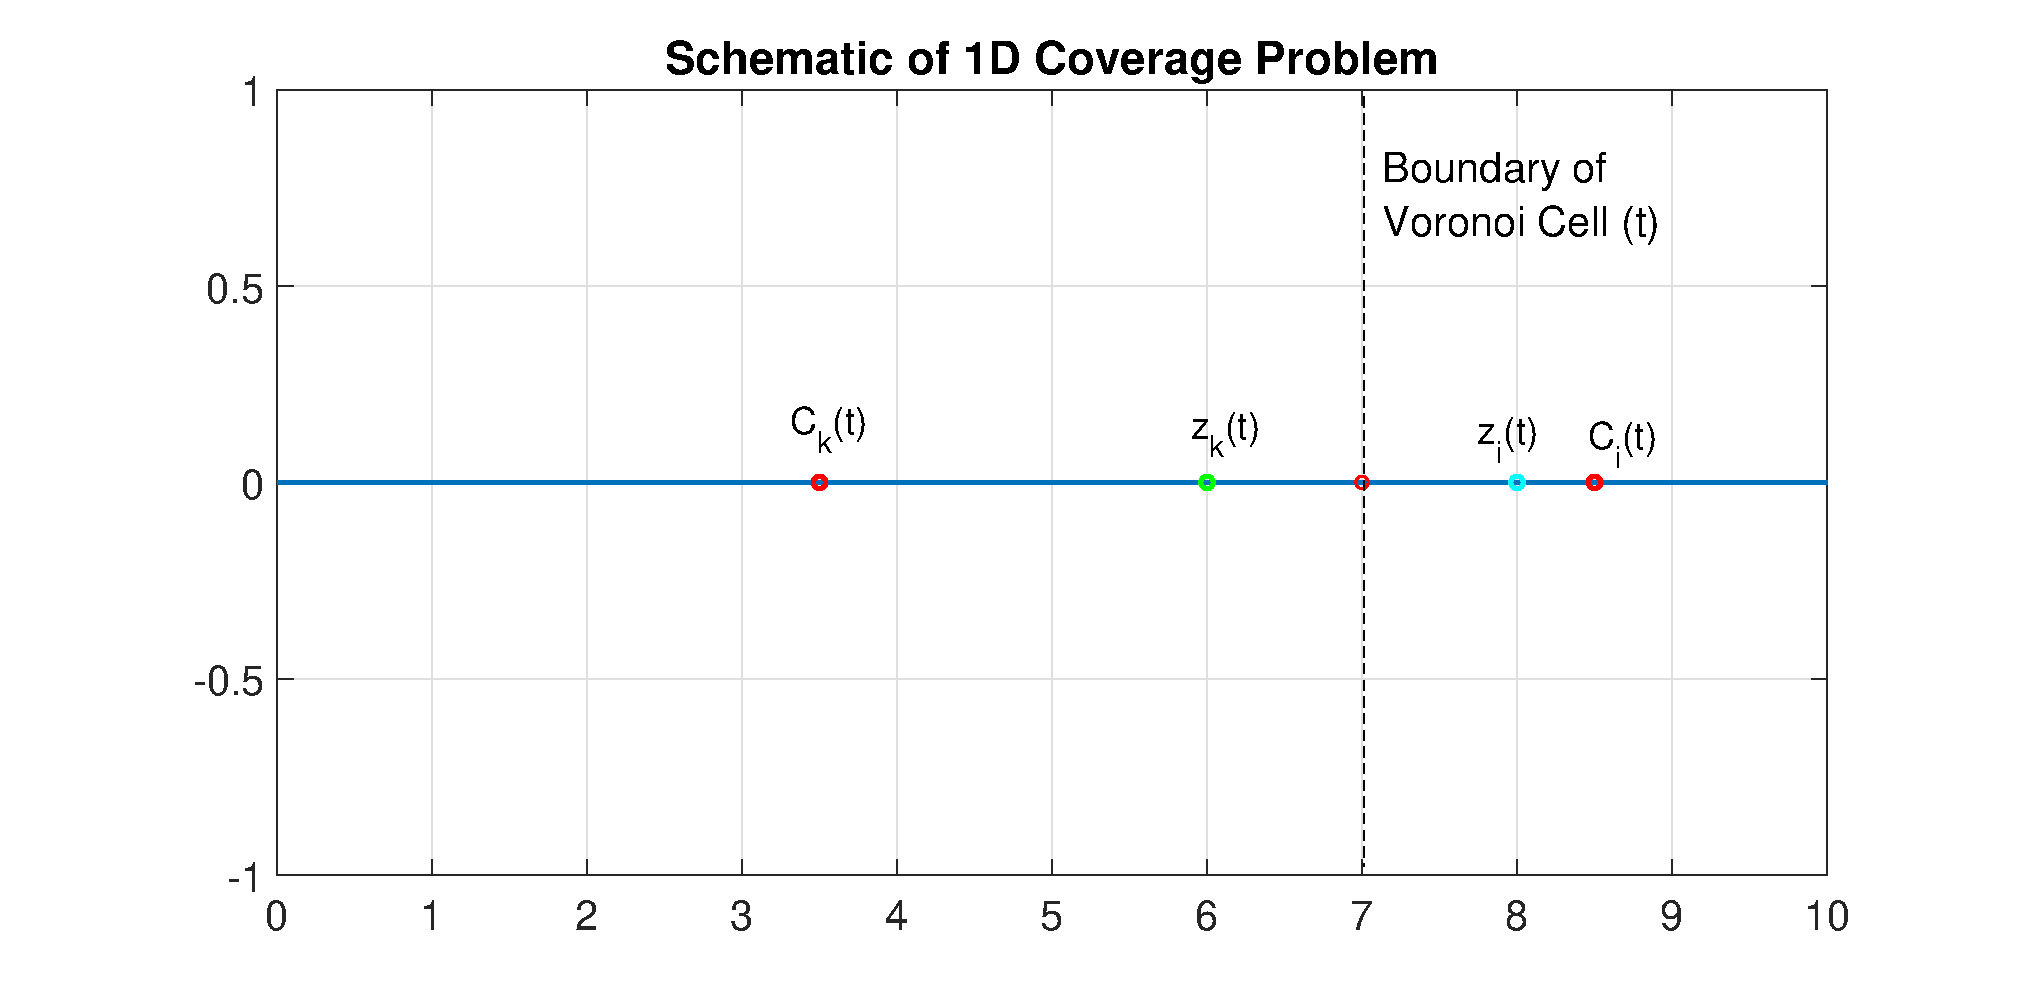
\includegraphics[width=1\linewidth]{Schematic_1D_Line}
	\caption{Schematic of 1D Coverage}
	\label{fig:Schematic_1D}
\end{figure}

\noindent Since the boundaries are fixed, the center mass $C_k$ depends only on the position of two agents. From the BLF in 2D Coverage Problem, we apply it for the 1D scenario.
\begin{equation}
V_k(Z(t)) = \displaystyle\sum_{j}^{} ln(\frac{b_j - a_jC_k(t)}{b_j - a_{j}z_{k}(t)})^2
\end{equation} 
where $j$ denotes the boundaries. From the definition of our Barrier Lyapunov Function, it has the following properties: \\
$\bullet$ $C_k(Z)$ is always the local optimum of the BLF. \\
$\bullet$ $C_k(Z)$ and $V_k(Z)$ are always well defined if the agents are always inside the interior of the coverage region. \\
There exists a descent direction of $V_k(Z)$ related to $z_k$, we use the convexity of the region to show that $z_k$ is still feasible if it follows this direction. Figure \ref{fig:BLF_2D_1} illustrates the descent direction of $V_k$. Note that the plot shows the contour of $V_k(Z)$, which depends on the position of both two agents and the green point is a vector notation that represents the position of two agents at any time.
\begin{figure} [!h]
	\centering
	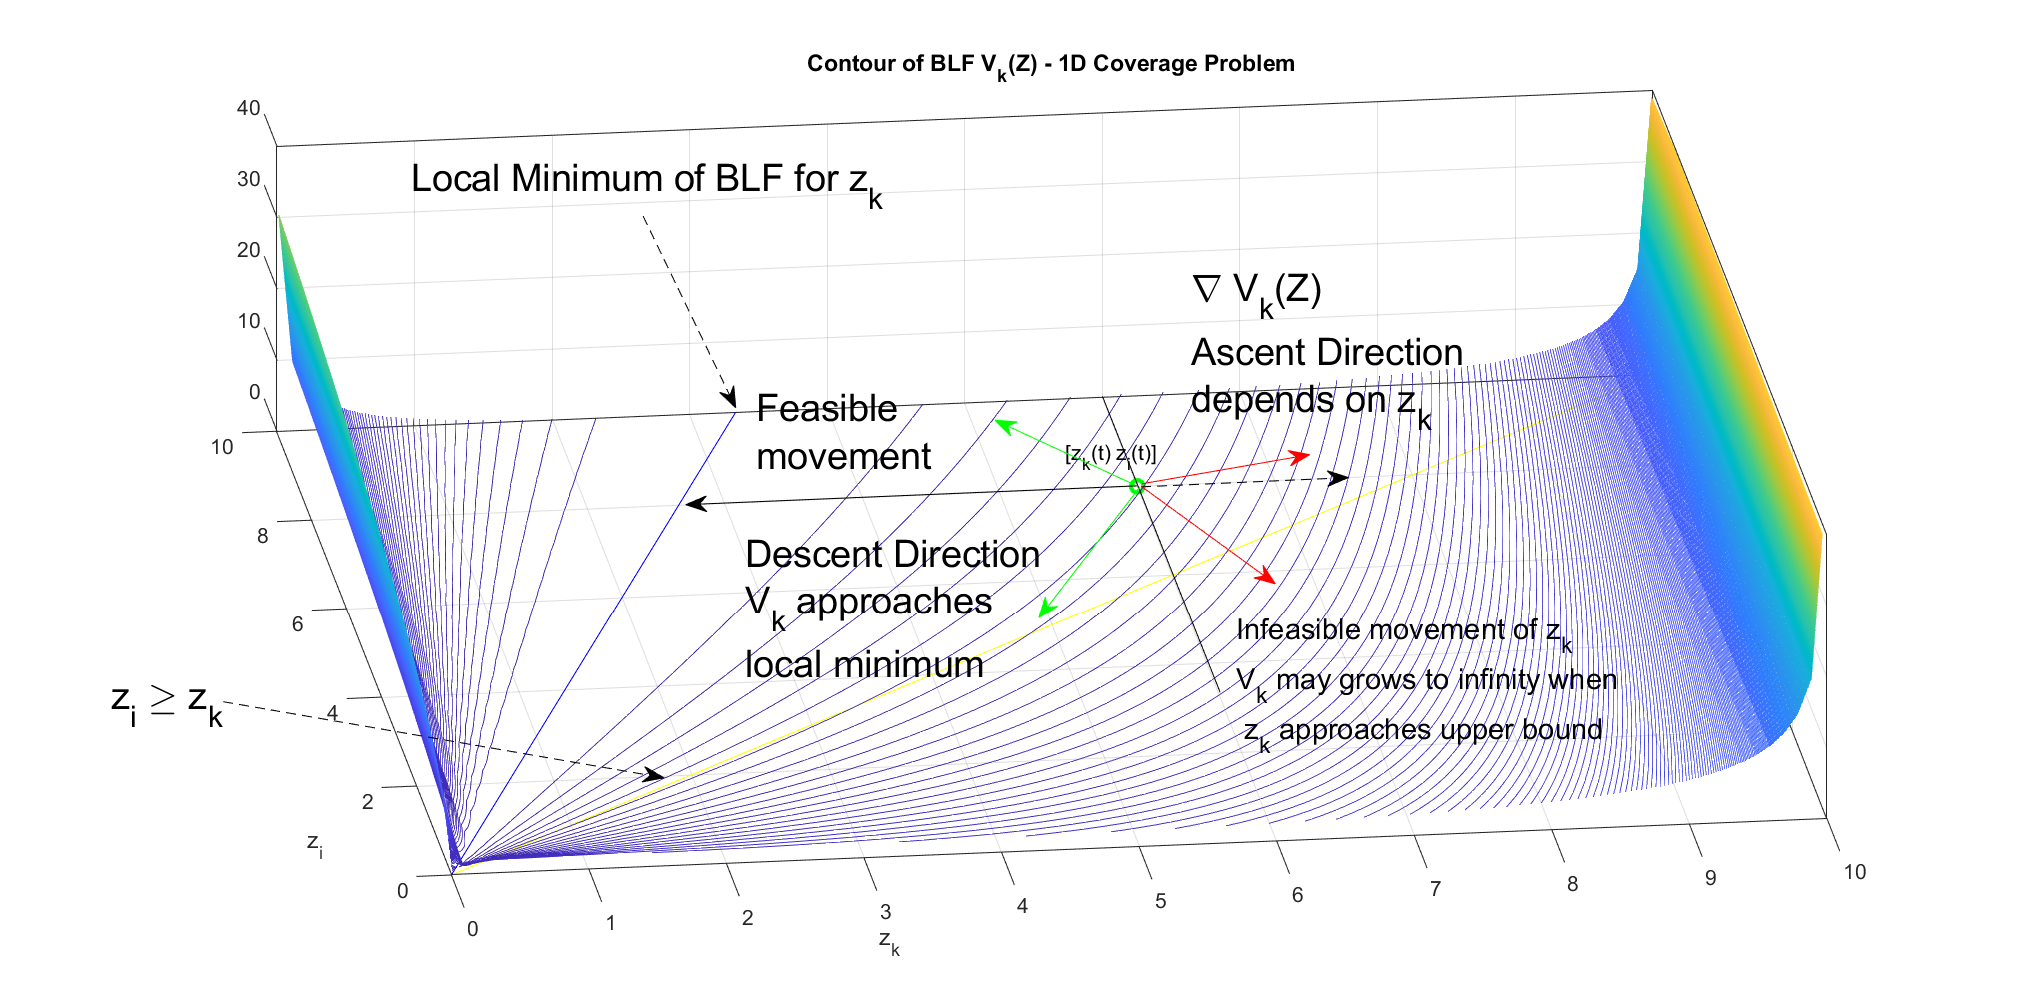
\includegraphics[width=1\linewidth]{Contour_1D_Coverage_Problem_BLF_zoom}
	\caption{Contour of BLF in 1D Coverage Problem}
	\label{fig:BLF_2D_1}
\end{figure}

\begin{figure} [!h]
	\centering
	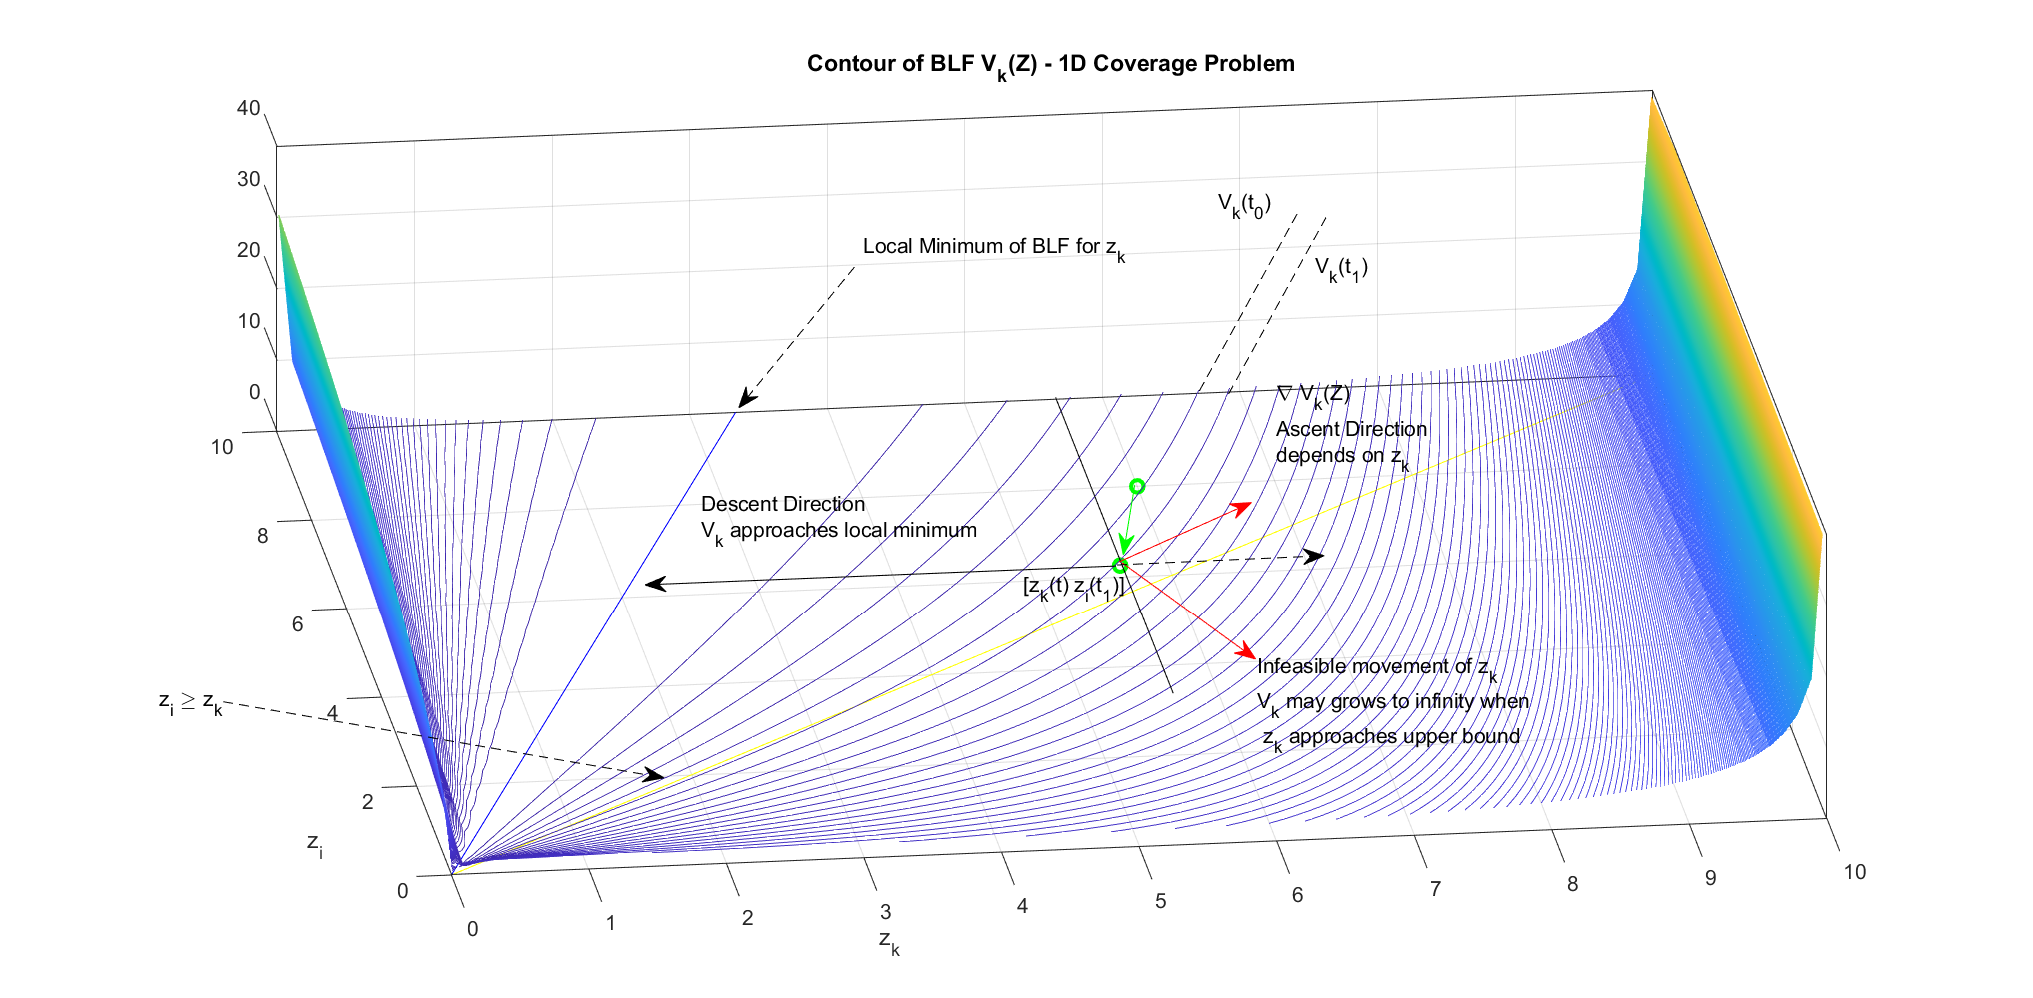
\includegraphics[width=1\linewidth]{BLF_1D_Coverage_Contour_Time_Evolution}
	\caption{Feasibility of Agent k in 1D Coverage Problem}
	\label{fig:BLF_2D_2}
\end{figure}
\noindent We observe that if $z_k$ always approaches $C_k$ by following the descent direction, it maintains inside the coverage region because the region is convex and $C_k$ is the local minimum of BLF. \\
Figure \ref{fig:BLF_2D_2} shows the time evolution of $z_k$. Even $z_k$ (x Axis) moves in the feasible direction, the BLF can still increase because the neighbor (y Axis) moves in the ascent direction related to $z_i$. Consequently, using this BLF alone can not solve the problem of coverage control because of the non-negative time derivative. However, what we need is just a feasible direction that guarantee the state constraints, and as long as all of the virtual masses keep moving, they converge to the set of centroidal Voronoi asymptotically. 




\chapter{Conclusion and Future Work}
%This thesis studied the problem of coverage control of a group of underactuated Wheeled Mobile Robots (WMR) under the state and input constraint. By applying a nonlinear scaling factor, the control law can handle input saturation to ensure the stability of the coverage problem. Besides, the thesis also proposed a switching condition, based on the theorem of barrier Lyapunov function, to guarantee that the state constraint is never violated. The method was proven and simulated under many scenarios with varying parameters and complexity. From a practical point of view, this control law is decentralized, applicable for any hardware specification of WMR, and for any convex coverage region. This corresponds to the motivation of the thesis that a control law can find a compromise to deal with all constraints at the same and ensure the operational performance. \\
%During the project, we note some challenges that open the potential research directions as future work. The first one refers directly to the proposed control law. By means of proposing a switching control, we do not consider the adjacent agents. Indeed, the movement of the neighbor agents is what makes the guarantee of the state feasibility challenging. Since the barrier Lyapunov function also depends on the position of these agents, we were not able to analyze the function analytically. This motivates us to find strategies that consider the uncertainties due to the neighbor agents to ensure all sufficient conditions of the proposition 2.\\
%One of the most important future work is conducting experiments to assess the control method. Since all the constraints considered in this project are strongly related to real situations, we are looking forward to evaluating the performance and the reliability from the practical aspect.\\
%Furthermore, the proposed controller has a limitation that it is only applicable to cover a convex region. Therefore, we are inspired to find a controller for a non-convex coverage that can also ensure all of the constraints. 

This thesis studies the problem of coverage control executed by a group of Wheeled Mobile Robots (WMR) under the state and input constraint. By applying a non-linear scaling factor, the control law can handle the input saturation to ensure the stability of the coverage problem. Besides, the thesis also proposes a switching condition, based on the theorem of barrier Lyapunov function, to guarantee that the state constraints are never violated. The method is proven and simulated under many scenarios with varying parameters and complexity. From a practical point of view, this control law is decentralized, applicable for any hardware specification of WMR,
and for any convex region. This corresponds to the motivation of the thesis that a control law can find a compromise to deal with all constraints at the same time and ensure the operational performance. \\
During the project, we note some challenges that open the potential research directions as future work. The first one refers directly to the proposed control law. By
means of applying a switching condition, we do not consider the adjacent agents. Indeed, the movement of the neighbor agents is what makes the guarantee of the state feasibility challenging. Since the barrier Lyapunov function also depends on the position of these agents, we were not able to analyze the function analytically. This motivates us to find strategies that consider the uncertainties due to the neighbor agents to ensure all sufficient conditions of the proposition 2. \\
One of the most important future work is conducting experiments to assess the control method. Since all the constraints considered in this project are strongly
related to real situations, we are looking forward to evaluating its performance and reliability from the practical aspect. \\
Furthermore, the proposed controller has a limitation that it is only applicable for convex regions. Therefore, we are inspired to find a control method for a non-convex coverage control that can ensure all of the constraints. \\


\appendix
	%_________Appendix__________________________________
\ifLSRITRtutorial
	\chapter{BUSTED! Last chance to actually read the HowTo-Section!!}
	
	Make sure your thesis is well structured, that each major section does what it is supposed to do, and that the whole thing hangs together. The basic structure is often as given in this template (but other structures are possible). In particular, don't think you need to have exactly as many major sections or chapters as the list implies; sometimes it makes sense to merge things, sometimes it makes sense to move things (e.g., the literature review is in many papers deferred until after the results), sometimes it makes sense to split a logical part into several individual sections. Just use some common sense.
	
	Hand in your thesis at minimum \textbf{one week} before the deadline for correction. You will receive feedback for the final version and very likely have to do minor or major revisions of your writing. Plan your writing schedule to allow for these adjustments, which can have quite some impact on your grade! 
	
	\optional{Please have a look on our \href{https://wiki.lsr.ei.tum.de/thesiswriting_students}{thesis-guidelines} as well before submitting your \emph{final} thesis.}
	
	\section{Style and Expressions}
	
	Before handing in your thesis, even for an intermediate review, please perform a spellcheck and correct grammar mistakes. The report is not meant to be a narrative text. Please stick to neutral and technical style and avoid subjective or biased expressions or adjectives/adverbs such as \emph{obviously, always, very, especially well, actually, so-called etc}. Scientific writing is about precision and you should underpin your statements factually, not soften them with unnecessary qualifiers.
	
	... Okay enough. But please check chapter \ref{sec:Tutorial} before starting with your report. 
\fi
%%%%%%%%%%%%%%%%%%_Abbildungsverzeichnis %%%%%%%%%%%%%%%%%%%%%%
\cleardoublepage
\addcontentsline{toc}{chapter}{List of Figures} 
\listoffigures 	

%%%%%%%%%%%%%%%%%%_List of Tables %%%%%%%%%%%%%%%%%%%%%%
% A lit of tables can be added - if wanted and needed by commenting out the lines below
% \cleardoublepage
% \addcontentsline{toc}{chapter}{List of Tables} 
% \listoftables	

%%%%%%%%%%%%%%%%%%_Acronyms and Notations %%%%%%%%%%%%%%%%%%%%%%
\cleardoublepage
%ifdefined\AddMyGloss
\AddMyGloss 
% --> see include/gloss.tex
%\fi

%%%%%%%%%%%%%%%%%%Literaturverzeichnis %%%%%%%%%%%%%%%%%%%%%%%%
\cleardoublepage
\addcontentsline{toc}{chapter}{Bibliography}
\begin{thebibliography}{9}
\bibitem{Qingchen} 
Qingchen Liu, Mengbin Ye, Zhiyong Sun, Jiahu Qin, and Changbin Yu.
\textit{Coverage control of unicycle agents under constant speed constraints}. 
IFAC-PapersOnLine, 50(1):2471{2476, 2017}.

\bibitem{Jorge} 
Jorge Cortes, Sonia Martinez, Timur Karatas, Francesco Bullo and \textit{Member IEEE}.
\textit{Coverage control for mobile sensing networks}. 
IEEE Transactions on Robotics and Automation.

\bibitem{Schwager} 
Mac Schwager.
\textit{A Gradient Optimization Approach to Adaptive Multi-Robot Control}. 
Ph.D. thesis, Massachusetts Institute of Technology.

\bibitem{Keng} 
Keng Peng Tee and Shuzhi Sam Ge
\textit{Control of Nonlinear Systems with Full State Constraint Using A
	Barrier Lyapunov Function}. 
Joint 48th IEEE Conference on Decision and Control and 28th Chinese Control Conference

\bibitem{Lee} 
Sung G. Lee and Magnus Egerstedt, Fellow, IEEE
\textit{Multi-Robot Control Using Time-Varying Density Functions}. 
IEEE Transactions on Robotic

\bibitem{ChengSong} 
Cheng Song, Lu Liu, Gang Feng.
\textit{Coverage control for homogeneous mobile sensors with input constraints on a unit circle}. 
Unmanned Systems, 4(01):15{21, 2016}.

\bibitem{Nguyen} 
Thien-Minh Nguyen, Xiuxian Li, Lihua Xie
\textit{Barrier Coverage by Heterogeneous Sensor Network with Input Saturation}. 
978-1-5090-1573-3/17/

\bibitem{Zhang} 
Zhang Jingxin, Zhou Pan, Ma Lei
\textit{Coverage Control of Multiple Heterogeneous Mobile Robots with Nonholonomic Constraints }. 
Proceedings of the 35th Chinese Control Conference

\bibitem{Zhang} 
Jun Xu, Jinwen Hu, Lihua Xie, Kai-Yew Lum
\textit{Distributed Coverage Control Under Generalized Locational Optimization Framework}. 
Proceedings of the 31st Chinese Control Conference

\bibitem{Flanders} 
Harley Flanders
\textit{Differentiation Under the Integral Sign}. 
The American Mathematical Monthly Vol. 80, No. 6 (Jun. - Jul., 1973), pp. 615-627

\bibitem{J. Wolff, M. Buss} 
J. Wolff, M. Buss
\textit{Invariance Control Design For Nonlinear Control Affine Systems Under Hard State Constraints}. 
IFAC Nonlinear Control Systems

\bibitem{Qiang Du} 
Qiang Du, Vance Faber and Max Gunzburger
\textit{Centroidal Voronoi Tessellations: Applications and Algorithms}. 
SIAM Review, Vol. 41, No. 4 (Dec., 1999), pp. 637-676

\bibitem{Qiang Du} 
Qiang Du; and Maria Emelianenko2;
\textit{Acceleration Schemes for Computing Centroidal Voronoi Tessellations}. 
NUMERICAL LINEAR ALGEBRA WITH APPLICATIONS. Numer. Linear Algebra Appl. 2006, 13 173 - 192

\bibitem{Song} 
Chanyoung Song, Jehyun Cha, Mokwon Lee, and Deok-Soo Kim
\textit{Dynamic Voronoi Diagram for Moving Disks}. 
DOI 10.1109/TVCG.2019.2959321, IEEE

\bibitem{Ichihara} 
Hiroyuki Ichihara, and Eitaku Nobuyama
\textit{Stability Analysis and Control Design of Linear Systems with Input Saturation Using Matrix Sum of Squares Relaxation}. 
5th IFAC Symposium on Robust Control Design

\bibitem{Takagi} 
Natsuki Takagi, Takeshi Nishida and Toshihiro Kobayashi
\textit{A Design of Adaptive Control Systems with Input Saturation}. 
SICE-ICASE International Joint Conference 2006

\bibitem{Chaoui} 
F. Z. Chaoui, F. Giri and M. M Saad
\textit{Adaptive Control in Presence of Input Saturation Constraint, an Input-Output approach}. 
1997 European Control Conference (ECC)

\bibitem{Valluri} 
Sairam Valluri and Vikram Kapila
\textit{Geometric Control of Input Saturated Systems with Guaranteed Closed-Loop Performance and Stability}. 
Proceedings of the American Control Conference

\bibitem{GENESIO} 
Min Cao and Christoforos Hadjicostis
\textit{Distributed Algorithms for Voronoi Diagrams and Applications in Ad-hoc Networks}. 

\bibitem{Sachan} 
Kapil Sachan and Radhakant Padhi
\textit{Barrier Lyapunov Function Based Output-constrained Control of Nonlinear Euler-Lagrange Systems}. 
2018 15th International Conference on Control, Automation, Robotics and Vision (ICARCV)

\bibitem{GENESIO} 
Roberto Genesio, Michele Tartaglia, Member IEEE and Antonio Vicino
\textit{On the Estimation of Asymptotic Stability Regions: State of the Art and New Proposals}. 
IEEE TRANSACTIONS ON AUTOMATIC CONTROL, VOL. AC-30. NO. 8, AUGUST 1985











\end{thebibliography}
 
%	\\ - [2] Cheng Song, Lu Liu, and Gang Feng. Coverage control for mobile sensor networks with input saturation. Unmanned Systems, 4(01):15{21, 2016.

%\bibliography{./refs/mybib}
\bibliographystyle{alphaurl}
%%%%%%%%%%%%%%%%%%%%License %%%%%%%%%%%%%%%%%%%%%%%%%%%%%%%%%%%
\cleardoublepage
\chapter*{License}
\markright{LICENSE}
This work is licensed under the Creative Commons Attribution 3.0 Germany
License. To view a copy of this license,
visit \href{http://creativecommons.org/licenses/by/3.0/de/}{http://creativecommons.org} or send a letter
to Creative Commons, 171 Second Street, Suite 300, San
Francisco, California 94105, USA.

%%%%%%%%%%%%%%%%%%%%List of TODOs %%%%%%%%%%%%%%%%%%%%%%%%%%%%%%%%%%%
% this MUST be empty and removed in the final version of course!
\listoftodos
\end{document}
